\chapter{Theory and methods}
\label{chap:theory}
%\begin{quote}
% \textit{This chapter discusses the theory of energy transfer.}
%\end{quote}
% 

\change{Heat transfer is customarily described theoretically either by monitoring the energy exchanged between individual atoms or by treating the heat carriers as a gas of particles flowing from hot to cold. While the particle picture is highly useful for, e.g., structures too large for atomic scale treatment, the structures considered in this thesis require atomic scale modeling capturing, e.g., the wave nature of phonons.}

This chapter reviews the microscopic theory and computational methods used in the thesis. Sections \ref{sec:th_eom1} and \ref{sec:th_eom2} present the relevant equations governing phononic, electronic and photonic energy transfer in microscopic scale. To highlight the common features in the modeling of different carriers, we start by postulating the Langevin equations of motion for the three carriers in Sec. \ref{sec:th_eom1}. Carrier-specific details and the derivation of the presented linearized equations are presented in \ref{sec:th_eom2}. 

Langevin theory is used throughout the thesis to model thermal fluctuations and dissipation, and this theory and the fluctuation-dissipation theorem are discussed in Sec. \ref{sec:th_langevin}. All calculations in the thesis aim at computing energy flow in the system, so the corresponding definitions of energy currents and their evaluation are reviewed in Sec. \ref{sec:th_currents}. Section \ref{sec:th_currents} also presents the spectral analysis methods developed in Publications \cp{spectral} and \cp{cnt} for determining frequency-wise contributions to interatomic energy transfer. \change{The evaluation of spectral energy current distribution in non-linear systems capturing phonon-phonon scattering requires monitoring dynamical correlations in atomic trajectories. The atomic trajectories are simulated with the classical molecular dynamics method, presented in Sec. \ref{sec:methods_md}.}


% Section \ref{sec:theory} presents the relevant equations governing phononic, electronic and photonic energy transfer in microscopic scale. We start by postulating the linear Langevin equations for the three carriers before moving to more in-depth derivations. We use Langevin theory \cite{langevin08} throughout this thesis to mathematically describe thermal fluctuations and the related dissipation. % After the minimal equations, the different carriers are discussed in more detail and 

%Because earlier parallel treatments (see, e.g., Ref. \cite{chen}) of the three carriers have mostly stressed the analogies in the energy transfer phenomena, we stress here the similarity of the Langevin equations of motion. The Langevin terms capture both thermal fluctuations and dissipation, necessary in modeling the creation and annihilation of energy carriers. 

% Section \ref{sec:methods} discusses the two methods used for solving the equations of motion in this thesis. The Green's function method solves the linear Langevin equations of motion in frequency domain so that by combining this solution with the fluctuation-dissipation theorem for the stochastic Langevin terms, one can calculate quantum-mechanical expectation values for observables such as the heat current flowing in the system. The second method is 

% Section \ref{sec:methods_mf} presents the classical molecular dynamics (MD) method, which is a powerful tool for simulating vibrational energy transfer in complex geometries. The main advantage of MD compared to GF method is the possibility to incorporate detailed phonon-phonon scattering mechanisms in the simulation, which is necessary in calculating phonon mean free paths in bulk materials or investigating the anharmonic contributions to interfacial energy transfer. Spectral analysis of energy currents is not, however, as straightforward with MD simulations as in the GF method, and one of the main goals of this thesis was to develop such analysis methods.

% We first review the classical molecular dynamics method, which was used to investigate lattice heat transfer in different geometries. Molecular dynamics allows for including non-linearities in the equations of motion, thereby accounting for detailed phonon-phonon interactions between different modes. Second approach to solving the equations of motion is the Green's function method, which requires, however, that the equations are fully linear \footnote{Keldysh Green's function methods \cite{haugjauho,wang08} can be used for perturbatively including non-linearities, but they are computationally heavy and therefore applicable only for relatively small systems.}. In this case, dissipative processes are captured by the effective relaxation rates introduced by the Langevin baths. The solution of Langevin equations of motion in terms of Green's functions is very similar for all three carriers, so the treatment is kept general when possible.
 
% Methods

% The role of Langevin baths

% 

\section{Langevin equations for phonon, photon and electron systems}
\label{sec:th_eom1}

\begin{figure}
 \begin{center}
 \end{center}
  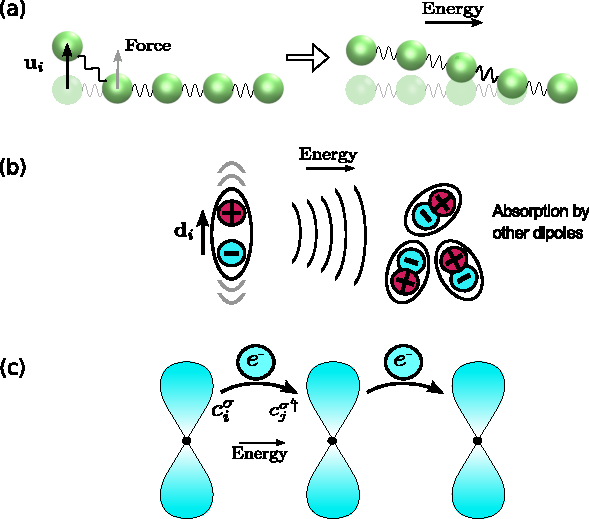
\includegraphics[width=.99\columnwidth]{inkscape/mechanisms.pdf}
 \caption{Schematic illustration of microscopic energy transfer mechanisms: (a) vibrational, (b) electromagnetic, and (c) electronic energy transfer. In phononic transfer, an atom $i$ displaced from its equilibrium position exerts a force on the neighboring atoms, giving rise to the propagation of displacement.}
 \label{fig:mechanisms}
\end{figure}
% This section reviews the general features of the Langevin equations of motion governing energy transfer by lattice vibrations, electromagnetic field, and electrons.
% allowing for simple but powerful modeling of energy transfer. 
\change{Langevin equations are a convenient and simple way to describe heat transfer in atomic scale, accounting for both wave dynamics and dissipation in carrier propagation}. This section reviews the general features of the Langevin equations of motion governing energy transfer by lattice vibrations, electromagnetic field, and electrons. The presented linearized equations for phononic, photonic and electronic energy transfer originate, respectively, from the works of Bolsterli, Rich and Visscher \cite{bolsterli70}, Rosa, Dalvit and Milonni \cite{rosa10,rosa11}, and Dhar, Sriram Shastry and Sen \cite{dhar03,dhar06b}. The derivation of the linearized equations from more general equations and the precise definitions of parameters are presented in Sec. \ref{sec:th_eom2}. % These equations are applied in this thesis for quantum-mechanical Green's function calculations of vibrational energy transfer through a point contact (\citepub{gf}) and electromagnetic energy transfer between nanoparticles in a microcavity (\citepub{dipole}). 

% Before writing down the equations of motion, we define the relevant degrees of freedom. 
Different energy transfer mechanisms and their corresponding degrees of freedom are schematically illustrated in Fig. \ref{fig:mechanisms}. Vibrational heat transfer in solids arises from the displacements $u_i^{\alpha}$ of each atom $i$ from their equilibrium positions to co-ordinate directions $\alpha\in\{x,y,z\}$. An atom displaced from its equilibrium position exerts a net force on other atoms, thereby leading to the propagation of displacement and transfer of energy. Similarly, electromagnetic energy is generated by fluctuations in local dipole moments $p_i^{\alpha}=qd_i^{\alpha}$, where $q$ is the dipole charge and $d_i^{\alpha}$ the dipole displacement in direction $\alpha$ \cite{rosa10}. The radiated electromagnetic energy propagates according to the Maxwell equations \cite{novotny}, scattered and absorbed by other dipoles. 

Quantum-mechanical electron transport in solids can be intuitively described by the tight-binding model \cite{ashcroftmermin}, in which electrons move by ''hopping'' between electron orbitals localized at individual atoms. Mathematically, the dynamics of a single electron is governed by the one-particle Schr\"odinger equation \cite{griffiths_qm}, but to capture fluctuations and dissipation, it is more practical to formulate the dynamical equations for electron creation and annihilation operators $c_i^{\sigma\dagger}$ and $c_i^{\sigma}$ \cite{ballentine}, which create and annihilate electrons at an orbital $\sigma$ localized at atom $i$, respectively\footnote{Label $\sigma$ is a composite index containing both the orbital wave function and electron spin.}. For notational simplicity, the same lattice subindex $i$ is used for each carrier to label the different spatial degrees of freedom. 
%  acting as electron creation and annihilation
\begin{figure}
 \begin{center}
 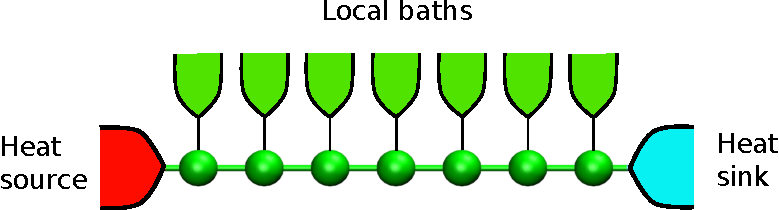
\includegraphics[width=.99\columnwidth]{pics/chain_baths.pdf}
 \caption{Schematic illustration of a chain of atoms coupled to Langevin baths. The baths at the left and right boundaries (red and blue) are at different temperatures and act as a heat source and sink, respectively. The baths colored in green describe internal fluctuations and dissipation arising from, e.g., phonon-phonon scattering.}
 \label{fig:langevin_chain}
  \end{center}
\end{figure}

Modeling of energy transfer requires coupling at least some of the degrees of freedom to external reservoirs acting as sources and sinks for energy. With the exception of \citepub{twinning}, where Nos\'e-Hoover thermostats \cite{nose84} are used, we employ Langevin baths as reservoirs in all works included in this thesis. The coupling of an atomic chain to Langevin baths is illustrated by a one-dimensional example in Fig. \ref{fig:langevin_chain}. In this case, the baths serve two purposes: The baths colored in red and blue act as external heat sources and sinks, respectively, and are used to drive energy through the system. The baths colored in green, on the other hand, mimic internal fluctuations and dissipation arising from anharmonic scattering, allowing for capturing non-linear effects in terms of effective relaxation rates \cite{bolsterli70}. This allows for a quantum-mechanical treatment of much larger systems than the more rigourous but computationally heavy Keldysh Green's function method \cite{haugjauho}, as discussed in more detail in \citepub{gf}. % In Publications \cp{fpu}, \cp{fpu2}, \cp{spectral}, \cp{cnt} and \cp{twinning}, non-linearities are captured by the molecular dynamics simulation and local heat baths are not used.

% For compact introduction, the linearized Langevin equation of motion governing each heat transfer mechanism is presented in Sec. \ref{sec:th_eom}. These equations for vibrational, electromagnetic and electronic energy transfer originate, respectively, from the works of Bolsterli, Rich and Visscher \cite{bolsterli70}, Rosa, Dalvit and Milonni \cite{rosa10,rosa11}, and Dhar, Sriram Shastry and Roy \cite{dhar03,roy07}. The derivation of the linearized equations from more general equations and their more detailed parameters are presented in Sec. \ref{sec:th_eom2}. The properties of the Langevin baths are discussed in Sec. \ref{sec:th_langevin}, where the fluctuation-dissipation theorems used for the calculation of expectation values are presented. The calculation of heat currents and its spectral decomposition into different frequency contributions are presented in Sec. \ref{sec:th_currents}.

% Thermal fluctuations and dissipation are captured in the linearized equations by Langevin terms allowing for including both quantum effects and dissipation. 

\subsection{Equations of motion: common features}
\label{sec:th_eom}

% Linearized stochastic equations of motion presented below allow for fully quantum-mechanical derivation of energy transfer rates and account for both wave effects and dissipation at the level of one-particle relaxation rates. These microscopic, Langevin equations of motion for vibrational, electromagnetic and electronic energy transfer originate, respectively, from the works of Bolsterli, Rich and Visscher \cite{bolsterli70}, Rosa, Dalvit and Milonni \cite{rosa10,rosa11}, and Dhar and Roy \cite{dhar03,dhar07}. All of these equations can be solved in a similar fashion, yielding frequency-resolved energy transfer rates in terms of Green's functions. Each of the equations is discussed in more detail in Sec. \ref{sec:th_eom2}, where also the steps leading to the linearized equations are presented and more references are given. % These equations have not been presented side-by-side in earlier literature. 
% This subsection presents the linearized Langevin equations of motion for phonon, photon, and electron systems and their respective degrees of freedom $\bu_i$, $\bb{d}_i$, and $c_i$. The compact form of these equations allows for highlighting the similarities in different transfer mechanisms and also gives a good overview of relevant quantities in each system. These Langevin equations are applied in this thesis for the Green's function calculations of vibrational energy transfer through a point contact and electromagnetic energy transfer in a microcavity, carried out in Publications \cp{gf} and \cp{dipole}, respectively.



% \change{Formally, the equations are of the form}
% \begin{equation}
%  \left\{ \begin{array}{c}
%           \textrm{Rate of} \\
% 	  \textrm{change} 
%          \end{array}
% \right\} \propto  \left\{ \begin{array}{c}
%           \textrm{Coupling } \\
% 	  \textrm{terms} 
%          \end{array}
% \right\}+
% \left\{ \begin{array}{c}
%           \textrm{Thermal} \\
% 	  \textrm{fluctuation} 
%          \end{array}
% \right\}+
% \left\{ \begin{array}{c}
%           \textrm{Dissipation} % \\
% 	    % as
%          \end{array}
% \right\}
% \end{equation}

The equations of motion for the three degrees of freedom $\bu_i$, $\bb{d}_i$, and $c_i^{\sigma}$ are all connected through the Langevin physics describing fluctuations and dissipation, leading to a similar solution methods and phenomenology despite involving different energy carriers. The equations read  \cite{bolsterli70,rosa10,rosa11,dhar03}
\begin{subequations}
\begin{align}
 m_i \ddot{\bu}_i(t) &=  - \sum_j \bb{K}_{ij}\bb{u}_j(t) + \xi_i(t) - m_i \gamma \dot{\bu}_i, \label{eq:th_eom1} \\
 m_i \ddot{\bb{d}}_i(t) &= - \sum_j \bb{K}_{ij} \bb{d}_j(t) +q\sum_{j} \bb{E}_{ij}(t)+\xi_i(t)+ q\Eenv(\br_i,t) - m_i \gamma \dot{\bd}_i(t), \label{eq:th_eom2}\\
 i\hbar \dot{c}_i^{\sigma}(t) &= -\sum_{j,\sigma'} t_{ij}^{\sigma\sigma'} c_j^{\sigma'}(t) +\eta_i^{\sigma}(t) - i\hbar \gamma_e c_i^{\sigma}(t) \label{eq:th_eom3}.
\end{align}
\end{subequations}
%The approximations leading to these equations are discussed in detail below in Sec. \ref{sec:th_eom2}, where also all the quantities are defined and the relevant references for these equations are given. 
Here $\bu_i=[u_i^{x},u_i^y,u_i^z]^T]$ and $\bd_i=[d_i^x,d_i^y,d_i^z]^T$ are written as three-dimensional vectors. Equations \eqref{eq:th_eom1}, \eqref{eq:th_eom2} and \eqref{eq:th_eom3} contain, generally speaking, four different kinds of parameters: inertial mass $m_i$ of atom or dipole $i$, coupling coefficients $\bb{K}_{ij}$, $\bE_{ij}$ and $t_{ij}^{\sigma\sigma'}$ coupling different degrees of freedom, Langevin noise terms $\xi_i$, $\eta_i$, and $\Eenv$ responsible for thermal fluctuations, and damping coefficients $\gamma$ and $\gamma_e$ accompanying the fluctuations according to the fluctuation-dissipation theorem (Sec. \ref{sec:th_langevin}). Noise terms $\xi_i$ and $\eta_i$ describe thermal fluctuations governed by Bose-Einstein and Fermi-Dirac statistics as detailed in Sec. \ref{sec:th_langevin}. The dipole equation of motion contains an additional noise term $q\Eenv(\br_i,t)$ arising from the thermal background electric field $\Eenv(\br_i,t)$, which must be included to ensure balance between electromagnetic absorption and emission in thermal equilibrium \cite{rosa10}.

% Formally, Eqs. \eqref{eq:th_eom1}, \eqref{eq:th_eom2} and \eqref{eq:th_eom3}

Equations \eqref{eq:th_eom1}, \eqref{eq:th_eom2} and \eqref{eq:th_eom3} are derived in more detail in Sec. \ref{sec:th_eom2}, but they can be easily understood intuitively. As an example, Eq. \eqref{eq:th_eom1} declares that the acceleration of atom $i$ is proportional to the sum of (i) the forces exerted by other atoms $j$, proportional for each atom pair $i,j$ to the force constant matrix $\bb{K}_{ij}$ calculated from interatomic potential energy, (ii) stochastic Langevin force $\xi_i$ modeling local thermal fluctuations, and (iii) friction term $m_i \gamma \dot{\bu}_i$ responsible for energy dissipation at rate $\gamma$. To highlight the similarities between different carriers, we have used the linear approximation for the interparticle force in equation \eqref{eq:th_eom1}, allowing for the direct solution of the equation of motion (see below). This assumption is relaxed in Sec. \ref{sec:th_eom2} to allow for more exact treatment of non-linear forces, which are responsible for microscopic phonon-phonon interactions and therefore necessary in the calculation of, e.g., frequency-dependent mean free paths (\citepub{cnt}) and the thermal conductivity of twinning nanowires (\citepub{twinning}). %The variance of the fluctuating force $\xi_i$ and the friction constant $\gamma$ are related by the fluctuation-dissipation theorem presented in Sec. \ref{sec:th_langevin}. 
% The detailed parameters of Eqs. \eqref{eq:th_eom1}, \eqref{eq:th_eom2} and \eqref{eq:th_eom3} are presented in Sec. \ref{sec:th_eom2}. 

It is worth noting that whereas equations \eqref{eq:th_eom1} and \eqref{eq:th_eom2} are purely real and involve second time-derivatives on the left-hand side, Eq. \eqref{eq:th_eom3} for the electron annihilation operator $c_i^{\sigma}$ is imaginary and involves only a single time-derivative. This difference is rooted in the fundamental property of quantum mechanics that time evolution is modeled by diffusion equation in imaginary time (Schr\"odinger equation), allowing for wave-like solutions in real time \cite{ballentine}.


% Detailed parameters and differences in Eqs. \eqref{eq:th_eom1}, \eqref{eq:th_eom2} and \eqref{eq:th_eom3} are presented in Sec. \ref{sec:th_eom2}.

% Equation of motion \eqref{eq:th_eom2} for the dipole moment $\bb{d}_i$ is similar to Eq. \eqref{eq:th_eom1}, but here the force exerted by dipoles $j$ is proportional to the electric fields $\bE_{ij}$, which is in turn linearly proportional to the dipole moment $\bp_j$. The local term $\bE_{ii}$ accounts for readiation reaction as discussed in Refs. \cite{rosa10,rosa11} and the oscillation parameter $\omega_0$ defines the resonance frequency. The relation of the Langevin equation of motion \eqref{eq:th_eom2} to the more commonly used fluctuating electrodynamics \cite{joulain05} is discussed in Sec. \ref{sec:th_eom2}. 

% In the Heisenberg equation of motion \eqref{eq:th_eom3} for electron annihilation operator, the dynamics of different orbitals are coupled by the tight-binding hopping constant $t_{ij}$ allowing for electron hopping between orbitals. The equation for the creation operator $c_i^{\dagger}(t)$ is obtained by taking the Hermitian conjugate of Eq. \eqref{eq:th_eom3}. 

\subsection{Solution of the Langevin equations in terms of Green's functions}
\label{sec:th_eom_solution}
The similarity of Eqs. \eqref{eq:th_eom1}, \eqref{eq:th_eom2}, and \eqref{eq:th_eom3} allows for solving the equations in a similar fashion. The differential equations are first turned in to algebraic equations by Fourier transforming the equations\footnote{We define Fourier transformation $\tilde f(\omega)$ for any function $f(t)$, as usual, as
\begin{equation}
 \tilde f(\omega) = \int_{-\infty}^{\infty} dt e^{i\omega t} f(t) \label{eq:th_fourier}
\end{equation}
and the corresponding inverse transformation as
\begin{equation}
 f(t) = \int_{-\infty}^{\infty} \frac{d\omega}{2\pi} e^{-i\omega t}\tilde f(\omega). \label{eq:th_fourier_inv}
\end{equation}}.
With small rearrangement, one then gets three linear systems of equations:
\begin{subequations}
\begin{align}
   - & \sum_{j,\beta}  [m_i (\omega^2+i\gamma \omega) \delta_{ij}\delta^{\alpha\beta} - K_{ij}^{\alpha\beta}] \tilde{u}_j^{\beta}(\omega) = \tilde \xi_i^{\alpha}(\omega) \label{eq:th_eom_fourier_phonon} \\
  - &  \sum_{j,\beta} \left[m(\omega^2+i\gamma\omega) \delta_{ij}\delta_{\alpha\beta} - K_{ij}^{\alpha\beta} +q^2 \omega^2 \mu_0 \mathbb{G}^{\alpha\beta}(\br_i,\br_j;\omega) \right]\tilde{d}_j^{\beta}(\omega) \notag \\
  & \qquad = q\tilde{E}_{\textrm{env}}^{\alpha}(\br_i,\omega) + \tilde{\xi}^{\alpha}_i(\omega) \label{eq:th_eom_fourier_photon} \\ 
  &  \sum_{j,\sigma'} \left[\hbar (\omega+i\gamma_e) \delta_{ij}\delta_{\sigma\sigma'} + t_{ij}^{\sigma\sigma'} \right] \tilde c_j^{\sigma'}(\omega) = \tilde \eta_i^{\sigma}(\omega)   \label{eq:th_eom_fourier_electron}
\end{align}
\end{subequations}
\change{where the Fourier-transformed degrees of freedom and Langevin noise terms are marked by tilde}. Angular frequency is denoted by $\omega$, Kronecker symbol $\delta_{ij}$ is zero for $i\neq j$ and equal to unity for $i=j$, and the co-ordinate directions $\alpha,\beta \in \{x,y,z\}$ are written explicitly in Eqs. \eqref{eq:th_eom_fourier_phonon} and \eqref{eq:th_eom_fourier_photon}. In Eq. \eqref{eq:th_eom_fourier_photon}, the Fourier transform $\tilde{\bE}_{ij}(\omega)$ of the electric field $\bE_{ij}$ appearing in Eq. \eqref{eq:th_eom2} is written in terms of the the electromagnetic Green's dyadic $\mathbb{G}^{\alpha\beta}(\br_i,\br_j;\omega)$ as \cite{novotny}
\begin{equation}
 \tilde{E}_{ij}^{\alpha}(\omega) = q\omega^2 \mu_0 \sum_{\beta} \mathbb{G}^{\alpha\beta}(\br_i,\br_j;\omega)\tilde{d}_j^{\beta}, \label{eq:th_Eij}
\end{equation}
where $\mu_0$ is the vacuum permittivity. The Green's dyadic $\mathbb{G}^{\alpha\beta}(\br_i,\br_j;\omega)$ is defined in Sec. \ref{sec:th_eom2_photon}. % In Eq. \eqref{eq:th_eom_fourier_photon}, the electromagnetic Green's dyadic $\mathbb{G}^{\alpha\beta}(\br_i,\br_j;\omega)$ \cite{novotny} describes the electromagnetic coupling of dipoles and is defined in \ref{sec:th_eom2_photon}. 

The linear systems of equations \eqref{eq:th_eom_fourier_phonon}, \eqref{eq:th_eom_fourier_photon} and \eqref{eq:th_eom_fourier_electron} can be written in matrix form by combining all degrees of freedom into single composite vectors by defining $\tilde{\bu}(\omega)=[u_1^x(\omega),u_1^y(\omega),u_1^z(\omega),u_2^x(\omega),u_2^y(\omega),u_2^z(\omega),\dots]^T$ and defining vectors $\tilde{\bd}(\omega)$ and $\tilde{\bb{c}}(\omega)$ similarly. The Langevin terms appearing on the right-hand sides of Eqs. \eqref{eq:th_eom_fourier_phonon}, \eqref{eq:th_eom_fourier_photon} and \eqref{eq:th_eom_fourier_electron} can be similarly written in vector form by accounting for the contribution of each bath $J$ on each degree of freedom. The bath label $J$ corresponds to either local baths, which contribute to the fluctuating force only at a single site, or the environment field $\tilde{E}_{\textrm{env}}^{\alpha}(\br,\omega)$. More details of the labeling are given, e.g., in \citepub{gf}.

Following such a procedure, each of the equations \eqref{eq:th_eom_fourier_phonon}, \eqref{eq:th_eom_fourier_photon}, and \eqref{eq:th_eom_fourier_electron} can be written in the matrix form
%he equations of motion \eqref{eq:th_eom_phonon_fourier}, \eqref{eq:th_eom_electron} and \eqref{eq:th_eom_dipoles} generally reduce to the matrix form
\begin{equation}
 \bb{A}(\omega) \tilde{\bb{x}}(\omega) = \sum_J \tilde \zeta^J(\omega). \label{eq:th_general}
\end{equation}
where $\bb{A}(\omega)$ is a coefficient matrix multiplying the degrees of freedom $\tilde{\bb{x}}(\omega)$ (standing for $\tilde{\bu}(\omega)$, $\tilde{\bb{c}}(\omega)$, or $\tilde{\bb{d}}(\omega)$ written in vector form) in Eqs. \eqref{eq:th_eom_fourier_phonon}, \eqref{eq:th_eom_fourier_photon}, and \eqref{eq:th_eom_fourier_electron}. The coefficient matrix $\bb{A}(\omega)$ captures all physical details of the system's deterministic dynamics, including coupling between different degrees of freedom and dissipation arising from the baths. The right-hand side of Eq. \eqref{eq:th_general} is the sum over stochastic Langevin forces $\zeta^J$ (standing for $\xi$, $\eta$, or $\Eenv$) from each bath $J$ as discussed above.  % To arrive at the matrix form, the site indices and coordinates have been combined into a single composite index. 

% The right-hand side of Eq. \eqref{eq:th_general} is the sum over stochastic Langevin forces $\zeta^J$ (standing for $\xi^J$, $\eta^J$, or $\Eenv$) from each bath $J$. The vectorized $\zeta^J$ is non-zero only at the sites that couple to the corresponding bath $J$. The bath index $J$ generally includes the baths coupled to each atomic site in the scattering region and, in case of phonons and electrons, baths representing external leads, which themselves consist of atoms coupled to Langevin baths at a prescribed temperature (and chemical potential for electrons). 

Equation \eqref{eq:th_general} can be solved by defining the Green's function as the matrix inverse $\bb{G}(\omega)=\bb{A}(\omega)^{-1}$ so that  
\begin{equation}
 \tilde{\bb{x}}(\omega)  =  \bb{G}(\omega) \sum_J \tilde \zeta^J(\omega). \label{eq:th_gf_solution}
\end{equation}
Equation \eqref{eq:th_gf_solution} can be straightforwardly interpreted: system's dynamics at each frequency is defined by the stochastic fluctuations from each bath at the same frequency, with the Green's function acting as the ''transfer matrix''. Our discrete formulation of the equations of motion allows for writing the Green's function as a matrix, but corresponding formulation for continuous medium would turn the Green's function into a function of two continous variables $\br$, $\br'$. In this case, matrix sums in Eqs. \eqref{eq:th_general} and \eqref{eq:th_gf_solution} would be replaced by an integral.

The matrix Green's function $\bb{G}(\omega)$ is generally of the form \cite{datta}
\begin{equation}
 \bb{G}(\omega) = \left[\bb{G}^0(\omega)^{-1} - \sum_J \Sigma^J(\omega) \right]^{-1},
\end{equation}
where $\bb{G}^0(\omega)$ is the Green's function in absence of dissipation (i.e., Langevin baths) and bath self-energy matrices $\Sigma^J(\omega)$ describe the dissipation and energy level renormalization arising from the interaction with each bath $J$. For example, the self-energy corresponding to the bath at site $k$, introducing a friction term $m_i\gamma \dot{\bu}_k$ in the equation of motion for $\bu_k$, is $[\Sigma(\omega)]_{ij}=-im_i\gamma \omega \delta_{ij} \delta_{ik}\unitdyadic$. Here $\unitdyadic$ is the $3\times3$ unit matrix. 

With the fluctuation-dissipation theorem for the force variances $\langle \zeta^J(\omega) \zeta^J(\omega')^T \rangle$ presented in Sec. \ref{sec:th_langevin} and the solution \eqref{eq:th_gf_solution} available, one can calculate the thermal averages of any observable of interest. The calculation of heat current $ Q_i^{\textrm{bath}}$ to bath $i$, which represents the locally dissipated power, leads to a Landauer-B\"uttiker-like expression \cite{landauer57,buttiker92} as outlined in Sec. \ref{sec:th_currents} and shown in detail in \citepub{gf}. % (see, e.g., Refs. \cite{dhar03} and \cite{dhar06})
% \begin{equation}
%   Q_I^{\textrm{bath}} = \int_0^{\infty} \frac{d\omega}{2\pi} \hbar \omega  \sum_J \ca{T}_{IJ}(\omega) \left[ f_{\textrm{BE}}(\omega,T_J)- f_{\textrm{BE}}(\omega,T_I)\right], \label{eq:th_QI}
% \end{equation}
% where the Bose-Einstein function is defined as
% \begin{equation}
%  f_{\textrm{BE}}(\omega,T)=\left[\exp(\hbar \omega/k_BT)-1\right]^{-1}, \label{eq:th_fBE}
% \end{equation}
% $T_I$ and $T_J$ are the temperatures of baths $I$ and $J$, and the transmission function between baths is defined as
% \begin{equation}
%  \ca{T}_{IJ}(\omega) = \textrm{Tr}\left[\Gamma^I(\omega) \bb{G}(\omega) \Gamma^J(\omega) \bb{G}(\omega)^{\dagger} \right]. \label{eq:th_caroli}
% \end{equation}
% Here $\Gamma^I(\omega)=-2\textrm{Im}[\Sigma^I(\omega)]$ is known as the bath coupling function \cite{datta}. Equation \eqref{eq:th_caroli} is the well-known Caroli form for the transmission function \cite{caroli71}, originally derived for ballistic two-terminal electron transport and later for phonons \cite{mingo06,yamamoto06}. In \citepub{dipole}, Eq. \eqref{eq:th_caroli} was shown to be valid also for electromagnetic energy transfer between a collection of dipoles. % The use of Eqs. \eqref{eq:th_QI} and \eqref{eq:th_caroli} for energy transfer calculations in different geometries is illustrated in Sec. \ref{sec:methods_gf}.
%  (corresponding to carrier annihilation) 
%\begin{subequations}
%\begin{align}
% m_i \ddot{\bu}_i &=  \bb{F}_i + \xi_i - m_i \gamma \dot{\bu}_i \\
% m \ddot{\bb{d}}_i &= - m\omega_0^2 \bb{d}_i + q\bb{E}_i+\xi_i - m_i \gamma \dot{\bu}_i \\
% i\hbar \dot{c}_i(t) &= -i\left[c_i,\ca{H}_{e}\right] +\eta_i - i\hbar \gamma_e c_i(t) 
%\end{align}
%\end{subequations}


\section{Equations of motion: Carrier-specific details}
\label{sec:th_eom2}

% This section reviews the equations of motion and their parameters for different carriers in more detail. General equations for lattice dynamics are given in Sec. \ref{sec:th_eom2_phonon}, where also the harmonic and anharmonic forces are defined. The microscopic theory of electromagnetic energy transfer starting from the Maxwell's equations is presented in Sec. \ref{sec:th_eom2_phonon}. Modeling of electron transfer by tight-binding model and Langevin theory as well as the assumptions underlying the linearized equation \eqref{eq:th_eom3} are briefly explored in Sec. \ref{sec:th_eom2_electron}.

% The linearized equations of motion presented in Sec. \ref{sec:th_eom1} are derived from more general equations and the parameters appearing in the equations are defined. 

% While the linearized Langevin equations of motion \eqref{eq:th_eom1}-\eqref{eq:th_eom3} act as a good starting point for energy transfer calculations, more sophisticated modeling is needed if the microscopic dynamics is to be treated more accurately. For the calculation of phonon mean free paths, for example, the detailed anharmonic interactions must be included in the model. In this case, Langevin terms are only used to feed and remove energy at the system boundaries. % The non-linearity of the equations of motion then forbids the direct solution of the equations of motion, so one has to resort to molecular dynamics simulations \cite{allentildesley} or perturbative first-principles calculations \cite{ziman}. 

%We start the discussion with vibrational heat transfer, where the general equations of motion, linearization of the equations and the definition of a phonon are introduced. We then continue to the electronic transport, where the tight-binding model is introduced. Because electronic transport plays a small role in this thesis, we only consider non-interacting electrons in order to keep the discussion brief. 

% Finally, we present the microscopic theory of electromagnetic energy transfer, starting from the Maxwell's equations of motion for the electric and magnetic fields. We show how the electric polarization acts as source term giving rise to thermal radiation. We also introduce the microscopic dipole model of Rosa, Dalvit and Milonni \cite{rosa10,rosa11} and compare it with the more traditional fluctuational electrodynamics \cite{rytov} approach often used for the modeling of electromagnetic energy transfer \cite{joulain05,volokitin07}. 

\subsection{Phonons}

\label{sec:th_eom2_phonon}
% \begin{figure}
% \begin{center}
%  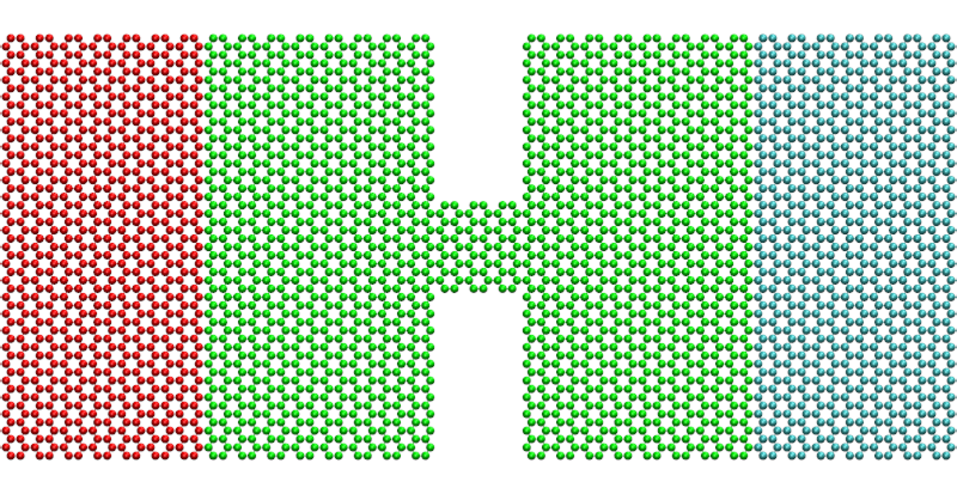
\includegraphics[width=.99\columnwidth]{pics/graphene_geom.pdf}
%  \caption{Schematic illustration of a point contact in graphene. The atoms colored in red and blue are assumed to be coupled to a heat source and sink, respectively, driving heat current through the point contact in the center region (green atoms). The thermalized regions extend infinitely far to the left and right}
% \label{fig:graphene_geom}
% \end{center}
% \end{figure} 

% As a concrete example of a phonon heat transfer problem, consider the constriction in graphene, depicted in Fig. \ref{fig:graphene_geom}. Graphene is a single sheet of carbon atoms arranged in a honeycomb lattice. The rigid $sp^2$ bonding of atoms and low defect density gives rise to high thermal conductivity \cite{ghosh08,balandin11}, making graphene an attractive material for extracting heat from electronic devices \cite{yan12}. In the shown geometry, the atoms colored in red and cyan are assumed to act as heat sources and sinks at high and low temperature, respectively. The thermalized regions are assumed to extend infinitely far to the left and right. 

We now move on to carrier-specific details leading to the linear Langevin equations \eqref{eq:th_eom1}, \eqref{eq:th_eom2}, and \eqref{eq:th_eom3}, starting from phonon heat transfer. The general equations of motion governing lattice dynamics are dictated by the lattice Hamiltonian \cite{ziman}
\begin{equation}
 \ca{H}_{\textrm{ph}} = \sum_{i=1}^N \frac{(\bp^{\textrm{kin}}_i)^2}{2m_i} + \ca{V}(\bb{r}_1,\dots,\bb{r}_N). \label{eq:th_hamiltonian}
\end{equation}
Here $\br_i$, $\bp^{\textrm{kin}}_i$, and $m_i$ are the position, kinetic momentum and mass of atom $i$, respectively\footnote{The notation $\bp_i$ is reserved for dipole moments.}. The total number of atoms (which can also be infinite) is denoted by $N$. The first term of Eq. \eqref{eq:th_hamiltonian} is the total kinetic energy of the atoms and the second term $\ca{V}$ is the interatomic potential energy responsible for the interatomic interactions. The choice of the potential energy function $\ca{V}$ is crucial for an accurate description of the lattice dynamics and, consequently, of energy transfer. In this thesis, we employed the Lennard-Jones \cite{allentildesley}, Tersoff \cite{tersoff88a}, Stillinger-Weber \cite{stillinger85}, and Fermi-Pasta-Ulam \cite{fermi55} potentials for modeling interatomic interactions in different systems.  %Models for $\ca{V}$ used in this work are presented in Publications \cp{fpu},\cp{fpu2}, \cp{spectral}, \cp{cnt}, and \cp{twinning} and in conjunction with the corresponding results in Chap. \ref{chap:results}.

Applying Hamilton's equations of motion $\dot{\br}_i=\partial \ca{H}_{\textrm{ph}}/\partial \bp_i^{\textrm{kin}}$ and $\dot{\bp}_i^{\textrm{kin}}=-\partial \ca{H}_{\textrm{ph}}/\partial \br_i$ \cite{fetter} accompanied by stochastic Langevin terms \cite{dhar06} gives the equations of motion
\begin{equation}
 m_i \ddot{\br}_i(t) = \bb{F}_i(t) + \xi_i(t) - m_i \gamma \dot{\bb{r}}_i(t), \label{eq:th_eom}
\end{equation}
where the deterministic force acting on atom $i$ is
\begin{equation}
 \bb{F}_i = - \frac{\partial \ca{V}}{\partial \bb{r}_i}. \label{eq:th_force}
\end{equation}
As discussed in Sec. \ref{sec:th_eom}, the Langevin terms $\xi_i$ and $m_i\gamma \dot{\bb{r}}_i$ generally have two roles in the modeling of heat transfer. They are used both for (i) coupling atoms located at system's boundaries to external heat sources and sinks,  and (ii) to describe dissipative processes, if non-linear interactions accounting for phonon-phonon interactions are neglected. The form of the friction term $m_i \gamma \dot{\bb{r}}_i(t)$, proportional only to instantaneous velocity, is called Ohmic due to its analogoue with a resistor in an electrical circuit \cite{weiss}. In general, the friction term is a time convolution giving rise to frequency-dependent damping \cite{weiss}, but in all publications included in this thesis, only the Ohmic form is used due to its simplicity.
 % The variance of the stochastic force $\xi_i$ determines the magnitude of oscillations and depends both on local bath temperature $T_i$ and friction parameter $\gamma$ through the fluctuation-dissipation relation discussed in Sec. \ref{sec:th_langevin}. 
% The stochastic Langevin force $\xi_i$ is a random variable with zero average and can be interpreted as phonon creation \cite{}. The variance of the stochastic force determines the magnitude of oscillations and depends both on bath temperature and friction parameter $\gamma$ through the fluctuation-dissipation relation discussed below in Sec. \ref{sec:th_langevin}. The friction term $m\gamma\dot{\bb{u}}_i$ damps oscillations and thereby accounts for phonon annihilation \cite{}. This form of friction, proportional only to instantaneous velocity, is called Ohmic due to its analogoue with a resistor in an electrical circuit \cite{weiss}. In general, the friction term is a time convolution giving rise to frequency-dependent damping \cite{weiss}, but in all publications included in this thesis, only the Ohmic form is used due to its simplicity.

Equation \eqref{eq:th_eom} generally describes the motions of atoms and molecules in solid, gas, and liquid systems. In solids, the atoms vibrate close to their equilibrium positions $\br_i^0$ and one can gain more insight into the lattice dynamics by focusing on the regime with small displacements from the equilibrium. The equilibrium positions $\br_i^0$ are defined by the condition of zero force:
\begin{equation}
 \left. \frac{\partial \ca{V}}{\partial \br_i} \right|_{\br_j=\br_j^0 \forall j} = 0. \label{eq:th_zeroforce}
\end{equation}
Assuming that the atoms remain close to the equilibrium positions, one can expand the potential energy in Taylor series in terms of the displacements $\bu_i=\br_i-\br_i^0$ \cite{ziman}:
\begin{equation}
 \ca{V} = \ca{V}_0 + \frac{1}{2} \sum_{i,j} \sum_{\alpha,\beta} u_i^{\alpha} K_{ij}^{\alpha \beta} u_j^{\beta}  + \frac{1}{6} \sum_{i,j,k} \sum_{\alpha,\beta,\gamma} \Upsilon_{ijk}^{\alpha\beta\gamma}  u_i^{\alpha} u_j^{\beta} u_k^{\gamma} + \mathcal{O}(u^4). \label{eq:th_V_taylor} % B_{ijk}^{\alpha\beta\gamma}
\end{equation}
In contrast to Eq. \eqref{eq:th_eom}, the Cartesian coordinate directions $\alpha,\beta \in \{x,y,z\}$ have been written here explicitly. The constant term $\ca{V}_0$ in Eq. \eqref{eq:th_V_taylor} does not play a role in dynamics, the first-order derivative term is zero due to Eq. \eqref{eq:th_zeroforce}, and the second-order term is proportional to the harmonic force constant (or ''spring'' constant) \cite{ziman}
\begin{equation}
 K_{ij}^{\alpha\beta} = \left. \frac{\partial^2 \ca{V}}{\partial u_i^{\alpha} \partial u_j^{\beta}} \right|_{\bu=\mathbf{0}}. \label{eq:th_K_def}
\end{equation}
The third term on the right-hand side of Eq. \eqref{eq:th_V_taylor} is proportional to the first-order anharmonic force constants
\begin{equation}
 \Upsilon_{ijk}^{\alpha\beta\gamma} = \left. \frac{\partial^3 \ca{V}}{\partial u_i^{\alpha} \partial u_j^{\beta} \partial u_k^{\gamma}} \right|_{\bu=\mathbf{0}}.
\end{equation}
These and higher-order anharmonic terms correspond to phonon-phonon interactions \cite{ziman} responsible for anharmonic scattering. First-principles calculation of thermal conductivities and phonon mean free paths requires explicitly including these terms in the equations of motion. The non-linearity of the resulting equations prevents, however, their direct solution, so one needs to turn either to computationally heavy Keldysh Green's function techniques \cite{wang08} or simulating lattice dynamics using the classical molecular dynamics (MD) method \cite{allentildesley}. MD is used in Publications \cp{spectral}, \cp{cnt}, \cp{twinning}, \cp{fpu}, and \cp{fpu2} due to its flexibility and applicability to large system sizes. MD is reviewed in Sec. \ref{sec:methods_md}.

%The third and fourth term on the right-hand side of Eq. \eqref{eq:th_V_taylor} are so-called anharmonic terms accounting for phonon-phonon interactions, which give rise to a finite thermal conductivity in infinite, perfect crystals \cite{ziman}. First-principles calculation of thermal conductivities and phonon mean free paths requires, therefore, including these terms in the equations of motion. The non-linearity of the resulting equations prevents their direct solution, so one needs to turn either to computationally heavy Keldysh Green's function techniques \cite{wang08} or simulating lattice dynamics using the classical molecular dynamics (MD) method \cite{allentildesley}. MD is used in Publications \cp{fpu}, \cp{fpu2}, \cp{twinning}, \cp{spectral}, and \cp{cnt} due to its flexibility and applicability to large system sizes and is reviewed in Sec. \ref{sec:methods_md}.

At sufficiently low temperatures or when dissipative events can be modeled in terms of a given relaxation time, anharmonic terms can be neglected. Including only the two first terms in the right-hand side of Eq. \eqref{eq:th_V_taylor} in the equation of motion \eqref{eq:th_eom} for the atomic displacement $\bu_i=\br_i-\br_i^0$ gives the system of linear equations \eqref{eq:th_eom1}, repeated here for convenience,
\begin{equation}
 m_i \ddot{\bu}_i(t) =  - \sum_j \bb{K}_{ij}\bb{u}_j(t) + \xi_i(t) - m_i \gamma \dot{\bu}_i.  \tag{\ref{eq:th_eom1}}
\end{equation}
The linearity of Eq. \eqref{eq:th_eom1} allows for direct solution in frequency domain as discussed in Sec. \ref{sec:th_eom_solution} and, consequently, including quantum statistics through the quantum fluctuation-dissipation theorem for the noise terms $\xi_i$ (Sec. \ref{sec:th_langevin}). 

% first-principles scattering rate calculations \cite{ziman},

%Applying the Fourier transformation and rearranging, the equations of motion \eqref{eq:th_eom1} reduce to a linear system of equations:
%\begin{equation}
% - \sum_{j,\beta}  [m_i (\omega^2+i\gamma \omega) \delta_{ij}\delta^{\alpha\beta} - K_{ij}^{\alpha\beta}] \tilde{u}_j^{\beta}(\omega) = \tilde \xi_i^{\alpha}(\omega) %\label{eq:th_eom_phonon_fourier}
%\end{equation}
%This linear equation can be straightforwardly solved in terms of the Green's function, defined as the inverse of the coefficient matrix multiplying $\tilde{u}_j^{\beta}(\omega)$. This procedure and the calculation of observables is discussed below in Sec. \ref{sec:th_gf}.

% In absence of dissipation ($\gamma=0$), the coefficient matrix of the system \eqref{eq:th_eom_fourier_phonon} is singular at frequencies corresponding to the system's eigenmodes, found by diagonalizing the matrix $D_{ij}^{\alpha\beta} = (m_i\omega^2 \delta_{ij}\delta^{\alpha\beta}-K_{ij}^{\alpha\beta})$. In a periodically repeating crystal, the eigenmodes can be labeled by the wavevectors $\bb{q}$ belonging to the first Brillouin zone \cite{ziman} and the branch $p \in \{1,\dots,3N_{\textrm{cell}}\}$, where $N_{\textrm{cell}}$ is the number of atoms in the unit cell. The eigenmodes are called phonon modes, while phonons are the discrete quanta of eigenmode occupation \cite{ziman}. The eigenfrequencies $\omega(\bb{q},p)$ form the phonon bandstructure, specifying the relation between the wavevectors and frequencies supporting propagating phonon modes. As an example, Fig. \ref{fig:th_nika} shows the phonon bandstructure of an infinite graphene sheet.
% 
% \begin{figure}
% \begin{center}
%  \includegraphics[width=8.6cm]{pics/nika09_fig3.pdf}
%  \caption{Phonon bandstructure of graphene, calculated using the valence force field method \cite{nika09}. The two-dimensional bandstructure is plotted along one-dimensional lines between special points in graphene reciprocal lattice, denoted by $\Gamma$, $M$ and $K$. Because graphene has two atoms per unit cell, there are altogether six phonon branches. The three branches that have vanishing frequencies at the $\Gamma$ point are called longitudinal acoustic (LA), transverse acoustic (TA) and out-of-plane acoustic (ZA). The optical modes LO, TO and ZO are labeled similarly. Reprinted with permission from Ref. \cite{nika09}.}
% \label{fig:th_nika}
% \end{center}
% \end{figure} 


% When both the anharmonic part in Eq. \eqref{eq:th_V_taylor} and the friction term proportional to $\gamma$ are neglected, the phonon eigenmodes are exact eigenmodes of the system and cannot dissipate their energy, giving rise to infinite thermal conductivity \cite{ziman}. In this thesis, we have included the important dissipative processes either by including the full anharmonic interactions or by including the friction term $\gamma$. In Publications \cp{fpu}, \cp{fpu2}, \cp{spectral}, \cp{cnt}, and \cp{twinning}, we have employed classical molecular dynamics simulations to account for anharmonic scattering, and therefore only the atoms coupled to ''hot'' and ''cold'' reservoirs are coupled to Langevin baths. In \citepub{gf}, on the other hand, anharmonic effects are mimicked by the interaction of all atoms with local Langevin baths. The linearity of the equations of motion then allows for, for example, accounting for quantum statistics. With the additional requirement of current conservation, this model is the so-called self-consistent heat bath model \cite{bolsterli70}. Molecular dynamics and the self-consistent heat bath model are explained in more detail below in Secs. XXX and XXX, respectively.

\subsection{Photons}
\label{sec:th_eom2_photon}
Energy transfer by electromagnetic waves is described by Maxwell equations \cite{jackson}. In the non-magnetic materials with no free charges as considered in this work, the electromagnetic fields arise from the fluctuating electric polarization fields inside the bodies, and the Maxwell equations for the electric field $\bE(\br,t)$ and magnetic field $\bb{H}(\br,t)$ read \cite{novotny}
\begin{subequations}
\begin{align}
  \nabla \times \bE(\br,t) + \mu_0 \frac{\partial \bb{H}(\br,t)}{\partial t} &= 0 , \label{eq:th_maxwell1} \\
  \nabla \times \bb{H}(\br,t) - \varepsilon_0 \frac{\partial \bb{E}(\br,t)}{\partial t} &=  \bb{j}(\br,t) , \label{eq:th_maxwell2} \\
   \nabla \cdot \bb{H}(\br,t) &= 0, \\
   \nabla \cdot \varepsilon_0 \bb{E}(\br,t) &= -\nabla \cdot \bb{P}(\br,t).
\end{align}
\end{subequations}
Here, $\mu_0$ and $\varepsilon_0$ are the magnetic permeability and permittivity of vacuum, respectively. The polarization current $\bb{j}(\br,t)=\partial \bb{P}(\br,t)/\partial t$ defined in terms of the polarization density $\bb{P}(\br,t)$ appears as a source term in Eq. \eqref{eq:th_maxwell2}, giving rise to an electromagnetic field according to Eqs. \eqref{eq:th_maxwell1} and \eqref{eq:th_maxwell2}. The radiated electromagnetic field carries an energy flux, whose magnitude and direction are given by the Poynting vector $\bb{S}(\br,t)=\bb{E}(\br,t)\times \bb{H}(\br,t)$ \cite{novotny}. The polarization density consists of stochastic and electrically induced contributions \cite{benabdallah11} as discussed below. 

% Written in this form, the equations are so-called macroscopic Maxwell equations \cite{novotny}, where the microscopic nature of matter is neglected and all fields are averaged over atomic scale variations. 

To derive an equation of motion for the electric field alone, let us calculate the curl of Eq. \eqref{eq:th_maxwell1}:
\begin{alignat}{2}
  \nabla \times \nabla \times \bE(\br,t) &= - \mu_0 \frac{\partial}{\partial t} \left[\nabla \times \bb{H}(\br,t) \right] 
\end{alignat}
By using Eq. \eqref{eq:th_maxwell2}, we get the Helmholtz equation for the electric field \cite{novotny}
\begin{equation}
   \nabla \times \nabla \times \bE(\br,t) + \mu_0 \varepsilon_0 \frac{\partial ^2\bb{E}(\br,t)}{\partial t^2}=  - \mu_0 \frac{\partial^2 \bb{P}(\br,t)}{\partial t^2}. \label{eq:th_eom_photons} % \label{eq:th_curlcurlE}
\end{equation}


% \begin{alignat}{2}
%  \nabla \times \nabla \times \bE(\br,t) &= - \mu_0 \frac{\partial}{\partial t} \left[\nabla \times \bb{H}(\br,t) \right] \\
%   &= - \mu_0 \varepsilon_0 \frac{\partial ^2\bb{E}(\br,t)}{\partial t^2} - \mu_0 \frac{\partial \bb{j}(\br,t)}{\partial t}. \label{eq:th_curlcurlE}
%  \end{alignat}
% Using the vector calculus identity $\nabla \times \nabla \times \bE(\br,t)=\nabla [\nabla \cdot \bE(\br,t)]-\nabla ^2\bE(\br,t)$ and defining the speed of light as $c=1/\sqrt{\varepsilon_0 \mu_0}$, one gets the Helmholtz equation for the electric field \cite{novotny}
% \begin{equation}
% \frac{1}{c^2} \frac{\partial ^2\bb{E}(\br,t)}{\partial t^2} = \nabla^2 \bE(\br,t) -\nabla (\nabla \cdot \bE)  - \mu_0 \frac{\partial^2 \bb{P}(\br,t)}{\partial t^2} \label{eq:th_eom_photons}
% \end{equation}

%This equation can be compared with the equation of elasticity for an isotropic continuum \cite{fetter}:
%\begin{equation}
%  \rho \frac{\partial^2 \bu(\br,t)}{\partial t^2} = \mu \nabla^2 \bu(\br,t) + \left(K+\frac{1}{3}\mu \right) \nabla[\nabla \cdot \bu(\br,t)] + \rho \bb{f}(\br,t). \label{eq:th_eom_ph_continuum}
%\end{equation}
%Here $\rho$ is the mass density, $\mu$ is the Lame coefficient, $K$ is the bulk modulus and, in contrast to Subsection \ref{sec:th_phonons}, the displacement $\bu(\br,t)$ is defined in continuum instead of lattice to make the analogy clear. The force $\bb{f}(\br,t)$ per unit mass, corresponding to Langevin fluctuations and dissipation in absence of external forces, plays a similar role in Eq. \eqref{eq:th_eom_ph_continuum} as a source of lattice vibrations as the second time derivative of polarization density $\bb{P}(\br,t)$ as a source of electromagnetic fields in Eq. \eqref{eq:th_eom_photons}.

To separate the fluctuating terms in the polarization density $\bb{P}(\br,t)$ in Eq. \eqref{eq:th_eom_photons}, let us divide the polarization density into the induced and fluctuating parts as $\bb{P}(\br,t)=\bb{P}_{\textrm{ind}}(\br,t)+ \bb{P}_{\textrm{fluc}}(\br,t)$. In the linear and local approximation, the induced part is proportional to the electric field in the frequency domain \cite{novotny}:
\begin{equation}
 \tilde{\bb{P}}_{\textrm{ind}}(\br,\omega)= \varepsilon_0 \chi(\br,\omega) \tilde{\bb{E}}(\br,\omega), \label{eq:th_P_chi}
\end{equation}
where $\chi(\br,\omega)$ is the susceptibility. The imaginary part of $\chi(\br,\omega)$ is responsible for dielectric losses \cite{jackson}. The fluctuating polarization density $\bb{P}_{\textrm{fluc}}(\br,t)$ is the analogue of the Langevin force and its variance in frequency-domain is proportional to the imaginary part of $\chi(\br,\omega)$ through the fluctuation-dissipation theorem presented in Sec. \ref{sec:th_langevin}.

Equation \eqref{eq:th_P_chi} lumps the complex response of the medium to the local electric field into a single, macroscopic parameter $\chi(\br,\omega)$. While such a macroscopic description has been used with great success to model energy transfer by electromagnetic fields in the framework of fluctuational electrodynamics \cite{rytov} (see, e.g., Refs. \cite{joulain05} and \cite{volokitin07} for reviews), \change{it is expected to break down in nanoscale} \cite{chalopin12b}. 

%and does not, therefore, allow for simultaneous coupling of optical and acoustic degrees of freedom as required, e.g., in the description of piezoelectric media \cite{}. In this thesis and \citepub{dipole}, we therefore turned to a more microscopic model for dipolar dynamics. % Other problems of the  (interaction of optical phonons with the electric field \cite{bornhuang})

A more microscopic model for fluctuating polarization fields was introduced by Rosa \textit{et al.} \cite{rosa10,rosa11} for the purpose of quantizing electromagnetic fields in lossy media. They modeled the polarization as a collection of dipoles $\bp_i$ located at points $\br_i$, corresponding to the dipole density
\begin{equation}
 \bb{P}(\br,t) = \sum_i \bp_i(t) \delta(\br-\br_i).
\end{equation}
The dynamics of each dipole was modeled by the classical oscillator model with mass $m_i$ and resonance angular frequency $\omega_0$ so that the equation of motion for the dipole displacement $\bd_i=\bp_i/q$ reproduces Eq. \eqref{eq:th_eom2} (with $K_{ij}^{\alpha\beta}=m\omega_0^2\delta_{ij}\delta_{\alpha\beta}$): \cite{rosa10,rosa11}
\begin{equation}
 m_i \ddot{\bb{d}}_i(t) = - m \omega_0^2 \bb{d}_i(t) +q\sum_{j} \bb{E}_{ij}(t)+\xi_i(t)+ q\Eenv(\br_i,t) - m_i \gamma \dot{\bd}_i(t). \label{eq:th_eom2b}
\end{equation}
The stochastic Langeving force $\xi_i$ and friction $m_i\gamma \dot{\bd}_i$ account for mechanical fluctuations and dissipation in dipole dynamics, respectively, and are equivalent to the corresponding Langevin terms in the phonon equation of motion \eqref{eq:th_eom}. The thermal background field $\Eenv(\br_i,t)$ acts as a similar noise term, corresponding to electromagnetic absorption of energy from the radiation field. To ensure balance between electromagnetic absorption and emission in thermal equilibrium, there must be an accompanying dissipative term in the equation of motion. Such a term is found in the local field $\bE_{ii}$, which manifests as Abraham-Lorentz radiation damping in the dipole motion \cite{jackson} as discussed in more detail in \citepub{dipole}. % In a fully optics-based treatment, the microscopicparameters $q$, $m_i$, and $\gamma$ do not need to be specified, because they can be absorbed into the definition of the local polarizability in the final results as described in Refs. \cite{rosa10,rosa11} and \citepub{dipole}. 

The local electric field $\bE_{ij}$ acting as a force term in Eq. \eqref{eq:th_eom2} and coupling different dipoles can be written in frequency-domain as [Eq. \eqref{eq:th_Eij}] \cite{novotny,rosa11}:
\begin{equation}
 %\tilde \bE(\br,\omega) = \tilde \bE_0(\br,\omega) + i \omega \mu_0 \int_V d\mathbf{r}' \mathbb{G}(\br,\br';\omega) \tilde{\bb{j}}(\br',\omega). \label{eq:th_Etilde}
\tilde \bE_{ij}(\omega) = \omega^2 \mu_0 \mathbb{G}(\br_i,\br_j;\omega) \tilde{\bb{p}}_j(\omega), \tag{\ref{eq:th_Eij}}
\end{equation}
where $\mathbb{G}(\br,\br';\omega)$ is the electromagnetic Green's dyadic found by solving Eq. \eqref{eq:th_eom_photons} in frequency-domain for a point-like dipole at $\br'$ \cite{novotny}:
 \begin{equation}
 \nabla \times \nabla \times \gem(\bb{r},\br';\omega) - (\omega^2/c^2) \epsenv(\br,\omega)\gem(\bb{r},\br';\omega)  =  \delta(\bb{r}-\br')\unitdyadic. \label{eq:intro_gemdef}
\end{equation}
The three-by-three unit dyadic is denoted by $\unitdyadic$. For generality, we have assumed that the point-like dipole is located in an inhomogeneous environment with dielectric constant $\epsenv(\br,\omega)$ to allow for modeling dipole-dipole energy transfer in a mirror cavity as in \citepub{dipole}. The calculation of Green's dyadics for planar multilayer geometries has been presented by Toma\v{s} \cite{tomas95}. By Fourier transforming Eq. \eqref{eq:th_eom2}, substituting Eq. \eqref{eq:th_Eij} and rearranging one gets the linear system of equations corresponding to Eq. \eqref{eq:th_eom_fourier_photon} for the dipole displacements:
\begin{alignat}{2}
 - & \sum_{j,\beta} \left[m(\omega^2-\omega_0^2+i\gamma\omega) \delta_{ij}\delta_{\alpha\beta} +q^2 \omega^2 \mu_0 \mathbb{G}^{\alpha\beta}(\br_i,\br_j;\omega) \right]\tilde{d}_j^{\beta}(\omega) \notag \\
  & \qquad = q\tilde{E}_{\textrm{env}}^{\alpha}(\br_i,\omega) + \tilde{\xi}^{\alpha}_i(\omega). \label{eq:th_eom_fourier_photon_b}
\end{alignat}

While Eq. \eqref{eq:th_eom_fourier_photon_b} is very similar to the corresponding (linearized) equation \eqref{eq:th_eom_fourier_phonon} for phonon heat transfer, there are some differences. In contrast to the static interatomic force constants $K_{ij}^{\alpha\beta}$ appearing in the phonon equation of motion, the dipole-dipole coupling coefficients $\mathbb{G}^{\alpha\beta}(\br_i,\br_j;\omega)$ are (i) frequency-dependent and (ii) depend on the electromagnetic environment through the dielectric constant $\epsenv(\br,\omega)$. Unlike lattice vibrations, electromagnetic energy can also propagate in vacuum. These differences are, however, related to our somewhat artificial separation between lattice vibrations and electromagnetic field. A fully coupled model of lattice vibrations and electromagnetic field \cite{chiloyan15} enables, e.g., tunneling of acoustic phonon energy across vacuum \cite{prunnila10}.

%\begin{alignat}{2}
% - & \sum_{j,\beta} \left[m(\omega^2-\omega_0^2+i\gamma\omega) \delta_{ij}\delta_{\alpha\beta} +q^2 \omega^2 \mu_0 \mathbb{G}^{\alpha\beta}(\br_i,\br_j;\omega) \right]\tilde d_j^{\beta}(\omega) \notag \\
%  &\qquad = q\tilde{\bE}_0^{\alpha}(\br_i,\omega) + \tilde{\xi}_i^{\alpha}(\omega) \label{eq:th_eom_dipoles}
%\end{alignat}

% Equation \eqref{eq:th_eom_fourier_photon} constitutes a closed set of linear equations that is analogous to Eqs. \eqref{eq:th_eom_fourier_phonon} and \eqref{eq:th_eom_fourier_electron}. Electromagnetic interactions between dipoles are captured by the Green's dyadic $\mathbb{G}^{\alpha\beta}(\br_i,\br_j;\omega)$, which plays the same role in electromagnetic energy transfer as the force constants $K_{ij}^{\alpha\beta}$ and hopping constants $t_{ij}$ play in vibrational and electron transfer, respectively. The Green's dyadic also accounts for the scattering of the electromagnetic field from the inhomogeneous environment, characterized by the dielectric constant $\epsenv(\br,\omega)$ appearing in Eq. \eqref{eq:intro_gemdef}. 

% With the frequency-domain solution \eqref{eq:th_gf_solution} for dipole moments and Eq. \eqref{eq:th_caroli} for locally absorbed power, one can calculate energy transfer rates between dipoles. \citepub{dipole} presented results for the thermal conductance between SiO$_2$ nanoparticles in a mirror cavity. Some of these results are summarized in Sec. \ref{sec:results_photon}. %As shown in Publication \citepub{dipole}, the transmission function \eqref{eq:th_caroli} can be expressed purely in terms of optical quantities, the local polarizability $\alpha_i(\omega)$ and electromagnetic Green's dyadic $\gem(\br,\br';\omega)$.

\subsection{Electrons}
\label{sec:th_eom2_electron}
 %Because we want to model electron creation and annihilation arising from fluctuations and dissipation, respectively, we formulate the model in terms of electron creation and annihilation operators \cite{ballentine}. 

First-principles modeling of electron transport starts from the quantum-mechanical Hamiltonian $\ca{H}_{\textrm{el}}$ for electrons and ions constituting the atomic lattice \cite{ashcroftmermin}. For the simplicity of discussion, we exclude electron-electron, electron-phonon, and electron-photon interactions so that the single-particle Hamiltonian for an electron moving in the periodic potential generated by the ions located at points $\bb{R}_i$ is \cite{ashcroftmermin}
\begin{equation}
 \ca{H}_{\textrm{el}} = - \frac{\hbar^2}{2m_e} \nabla^2  + \sum_i V(\br-\bb{R}_i), \label{eq:th_Hel}
\end{equation}
where $m_e$ is the electron mass and $V(\br-\bb{R}_i)$ is the screened electrostatic potential from ion $i$. To arrive at the tight-binding approximation, we first solve the energy levels and eigenstates $\phi_i^{\alpha}(\br)$ for a \textit{single} ion:
\begin{equation}
 \left[ - \frac{\hbar^2}{2m_e} \nabla^2  +  V(\br-\bb{R}_i) \right] \phi_i^{\sigma} (\br) = E_i^{\sigma} \phi_i^{\sigma}(\br) \label{eq:th_schrode}
\end{equation}
The localized solutions of Eq. \eqref{eq:th_schrode} are centered around $\bb{R}_i$ due to the attractive ion potential $V(\br-\bb{R}_i)$. The tight-binding approximation is to assume that the localized orbitals $\phi_i^{\sigma}$ for each atom $i$ form a complete set \footnote{Typically only a small subset is used, as tightly bound states do not need to be included. More generally, Wannier functions can be used as basis functions \cite{ashcroftmermin}.} so that the electron eigenstates of Hamiltonian \eqref{eq:th_Hel} can be written as
\begin{equation}
 \psi(\br) = \sum_{i,\sigma} b_i^{\sigma} \phi_{i}^{\sigma}(\br).
\end{equation}
Assuming for simplicity that the overlap matrix element $\langle \phi_i^{\sigma}| \phi_j^{\sigma'} \rangle$ is negligible compared to unity for $i\neq j$, one can approximate the Hamiltonian matrix elements of the basis functions to be
\begin{equation}
 \langle \phi_i^{\sigma} | \ca{H}_{\textrm{el}} | \phi_j^{\sigma'} \rangle \approx E_i^{\sigma} \delta_{ij}\delta_{\sigma\sigma'}  - \tilde t_{ij}^{\sigma\sigma'}, \label{eq:th_Helements}
\end{equation}
where the ''hopping'' matrix element is 
\begin{equation}
  \tilde t_{ij}^{\sigma\sigma'} = - \int d\bb{r} \phi_i^{\sigma}(\br)^*  \sum_{k\neq j} V(\br-\bb{R}_k)   \phi_j^{\sigma'}(\br).
\end{equation}
The tight-binding Hamiltonian with the matrix elements of Eq. \eqref{eq:th_Helements} can then be written in the braket notation \cite{schwabl} as 
\begin{equation}
 \ca{H}_{\textrm{el}}^{\textrm{tb}} = \sum_{i,j} \sum_{\sigma,\sigma'} (E_i^{\sigma} \delta_{ij}\delta_{\sigma\sigma'}  - \tilde t_{ij}^{\sigma\sigma'})|\phi_i^{\sigma} \rangle \langle \phi_j^{\sigma'} | \label{eq:th_Hel_tb}
\end{equation}
The equivalent second-quantized form \cite{schwabl} for the Hamiltonian \eqref{eq:th_Hel_tb} is
\begin{equation}
 \ca{H}_{\textrm{el}}^{\textrm{tb}} = \sum_{i,j} \sum_{\sigma,\sigma'} (E_i^{\sigma} \delta_{ij}\delta_{\sigma\sigma'}  - \tilde t_{ij}^{\sigma\sigma'}) c_i^{\sigma\dagger} c_j^{\sigma'} \label{eq:th_Hel_tb_final}
\end{equation}
where the electron creation operator $c_i^{\sigma\dagger}$ creates an electron in orbital $\phi_i^{\sigma}$ and annihilation operator $c_j^{\sigma'}$ annihilates electrons at orbital $\phi_j^{\sigma'}$:
 \begin{subequations}
  \begin{align} 
     c_i^{\sigma\dagger} |0 \rangle = | \phi_i^{\sigma} \rangle,  \\
     c_j^{\sigma'} |\phi_j^{\sigma'} \rangle = | 0 \rangle.
  \end{align}
 \end{subequations}
Here $|0\rangle$ is the vacuum state with no electrons. 

%The tight-binding Hamiltonian \eqref{eq:th_Hel_tb_final} can also be derived from spatial discretization of the one-particle Schr\"odinger equation \eqref{eq:th_schrode}, in which case the index $i$ labels the discretization grid points \cite{datta}. \textbf{CLARIFY}


% The hopping constant $t_{ij}$ allows for electron hopping between orbitals $i$ and $j$ and can be calculated from the Hamiltonian matrix element \cite{ashcroft}
% \begin{equation}
%  t_{ij} = - \int d\br \psi_i(\br)^*  \Delta U(\br)  \psi_j(\br) ,
% \end{equation}
% where $\Delta U(\br) $ is the ''perturbation'' Hamiltonian 

% The local term $t_{ii}$ in Eq. \eqref{eq:th_Hel} accounts for variations in the local potential created by, e.g., external electric fields \cite{datta}. %For graphene, the hopping constant between nearest-neighbor carbon atoms is approximately $2.5$ eV \cite{dassarma11}.

With the Hamiltonian of Eq. \eqref{eq:th_Hel_tb_final}, the Heisenberg equation of motion $i\hbar \dot{c}_i^{\sigma} = - \left[\ca{H}_{\textrm{el}}^{\textrm{tb}},c_i^{\sigma} \right]$ \cite{ballentine} accompanied by the stochastic Langevin force $\eta_i^{\sigma}$ and Ohmic damping $-i\hbar \gamma_e c_i^{\sigma}(t)$ \cite{dhar03} leads to the equation of motion \eqref{eq:th_eom3}, reproduced here:
\begin{equation}
 i\hbar \dot{c}_i^{\sigma}(t) = -\sum_{j,\sigma'} t_{ij}^{\sigma\sigma'} c_j^{\sigma'}(t) +\eta_i^{\sigma}(t) - i\hbar \gamma_e c_i^{\sigma}(t) \tag{\ref{eq:th_eom3}}.
\end{equation}
Here the orbital energy $E_i^{\sigma}$ was absorbed to the hopping constant through the definition 
\begin{equation}
 t_{ij}^{\sigma\sigma'}=\tilde t_{ij}^{\sigma\sigma'}-E_{i}^{\sigma}\delta_{ij}\delta_{\sigma\sigma'}.
\end{equation}

% Fourier transform and rearranging gives the linear system of equations \eqref{eq:th_eom_fourier_electron}. 

The Langevin terms $\eta_i^{\sigma}$ and $-i\hbar \gamma_e c_i^{\sigma}$ in Eq. \eqref{eq:th_eom3} are responsible for creating and annihilating electrons, respectively, and thereby act essentially as additional scattering channels. This idea of modeling inelastic effects by additional scattering channels is due to B\"uttiker \cite{buttiker86} and d'Amato and Pastawski \cite{damato90}, and it greatly simplifies the modeling of dephasing and dissipation events in quantum transport compared to the more rigorous but computationally demanding perturbative Keldysh Green's function techniques \cite{haugjauho}. % The relation between scattering channels and Langevin dynamics was noted by Dhar and Sriram Shastry \cite{dhar03}. % B\"uttiker's voltage probe model is, in turn, closely related to the self-consistent heat bath model introduced 15 years earlier by Bolsterli, Rich and Visscher \cite{bolsterli70}. 

Equation \eqref{eq:th_eom3} is formally similar to the phonon equation of motion \eqref{eq:th_eom1}, with the hopping constants $t_{ij}^{\sigma\sigma'}$ playing the role of force constants $K_{ij}^{\alpha\beta}$. Differences arise from, e.g., the first-order time derivative in the equation for electrons. As a consequence, there is no simple correspondence between the electron dynamics at energies $E$ and $-E$ [described by the terms $c_i^{\sigma}(E/\hbar)$ and $c_i^{\sigma}(-E/\hbar)$] whereas for phonons, one can restrict the analysis to positive frequencies due to the identity $\tilde{\bu}_i(\omega)^*=\tilde{\bu}_i(-\omega)$. As a second difference, electron occupation at thermal equilibrium obeys Fermi-Dirac statistics with chemical potential $\mu$ and temperature $T$, which is evident in the fluctuation-dissipation theorem discussed in Sec. \ref{sec:th_langevin}. As is well-known \cite{ashcroftmermin}, only electrons with energies close to $\mu$ participate in transport, and this narrow-energy band enables relatively easy control of electron flow. For phonons, the statistics at thermal equilibrium is Bose-Einstein distribution with the chemical potential $\mu=0$. As a consequence, thermal transport by phonons is always broadband with a large range of frequencies \footnote{Except at very low temperatures, where only a narrow range of phonons close to the zero-frequency can be excited.} \cite{ziman}. %\change{Therefore, electronic transport can be typically controlled more easily than phonons.}

% Equation \eqref{eq:th_eom_fourier_electron} is very similar to the phonon equation \eqref{eq:th_eom_fourier_phonon}. The stochastic Langevin terms appear as source terms on the right-hand side of the equation and the friction term shifts the eigenfrequencies away from the real axis by introducing dissipation. The interatomic force constant $K_{ij}^{\alpha\beta}$ plays the same role in coupling atomic vibrations as the coupling constant $t_{ij}$ does in allowing electron hopping. 


%\begin{equation}
% i \hbar \dot{c}_i(t) = - \sum_{j} t_{ij} c_j(t) + \eta_i(t) - i\hbar \gamma_e c_i(t). \label{eq:th_eom_electron_t}
%\end{equation}
%Fourier transformation and rearranging leads to the system of equations:
%\begin{equation}
% \sum_{j} \left[\hbar (\omega+i\gamma_e) \delta_{ij} + t_{ij} \right] \tilde c_j(\omega) = \tilde \eta_i(\omega) . \label{eq:th_eom_electron}
%\end{equation}




%The Langevin coupling introduced in Eq. \eqref{eq:th_eom_electron_t} is closely related to the B\"uttiker voltage probe \cite{nazarov}, introduced by B\"uttiker \cite{buttiker86} to investigate the effects of inelastic scattering and dephasing on quantum transport. 


% Analogy with \eqref{eq:th_eom_phonon_fourier}




%The solution of these equations in terms of the Green's functions and the calculation of observables such as heat currents is described in Sec. \ref{sec:methods}.

%For atomic displacements $\bu_i$, we also employ the full equation of motion \eqref{eq:th_eom} to capture non-linearitites corresponding to phonon-phonon interactions in vibrational energy transfer. The non-linearities prevent a direct solution of the equations of motion, so classical molecular dynamics simulations \cite{allentildesley} are used to calculate heat currents. MD simulations are discussed below in Sec. \ref{sec:methods}

\section{Langevin theory}
\label{sec:th_langevin}
% This section reviews the statistical properties of the Langevin terms $\xi_i$, $\eta_i$ and $\Eenv$ in more detail, as required for the Green's function calculations of energy currents  (Publications \cp{gf} and \cp{dipole}) and simulating classical Langevin dynamics in MD (Publications \cp{fpu}, \cp{fpu2}, \cp{spectral}, \cp{cnt}). 

As noted earlier, Langevin theory is used throughout this thesis to model thermal fluctuations. In the classical Langevin theory, the system under study is imagined to interact with an infinite collection of harmonic oscillators. With a few simplifying assumptions \cite{weiss}, one can integrate out the bath degrees of freedom so that their interactions with the system are effectively described by fluctuating and dissipative forces \cite{weiss,dhar06}. The fluctuating force is a random variable with zero average and its variance is fixed by the fluctuation-dissipation theorem (FDT) \cite{nyquist28,callen51}, which relates the strength of fluctuations to the dissipation. FDT essentially ensures the onset of statistical thermal equilibrium when all bath temperatures are equal.

%  (and chemical potential in case of electrons)

For Ohmic coupling to a bath of harmonic oscillators, assumed for atomic displacements in Eqs. \eqref{eq:th_eom1} and dipole displacements in Eq. \eqref{eq:th_eom2}, the variance of the Langevin force $\tilde{\xi}_i$ in frequency domain is related to the friction parameter $\gamma$ and bath temperature $T_i$ through the FDT \cite{weiss,dhar06}
\begin{equation}
 \langle \tilde \xi_i(\omega) \tilde \xi_i(\omega')^T \rangle = 4\pi \delta(\omega+\omega') \hbar \omega m_i \gamma \left[f_{\textrm{BE}}(\omega,T_i)+ \frac{1}{2} \right] \bb{I}_{3\times 3}. \label{eq:th_xixiom_ohmic_qm}
\end{equation}
Here the angular brackets stand for statistical ensemble average, the Bose-Einstein function is defined as
\begin{equation}
 f_{\textrm{BE}}(\omega,T)=\left[\exp(\hbar \omega/k_BT)-1\right]^{-1}, \label{eq:th_fBE}
\end{equation}
and the unit matrix $\unitdyadic$ reflects the independence of fluctuations in different coordinate directions. For the Ohmic coupling of electrons to a bath, the variance of the ''force'' $\tilde{\eta}_i$ appearing as a source term in Eq. \eqref{eq:th_eom3} is \cite{dhar03,dhar06b,roy07}
\begin{equation}
 \langle \tilde \eta_{i}^{\sigma\dagger}(\omega) \tilde \eta_{j}^{\sigma}(\omega') \rangle = 4\pi\delta(\omega-\omega') \gamma_e f_{\textrm{FD}}(\omega;\mu_{i},T_{i}) \delta_{ij}\delta_{\sigma\sigma'}, \label{eq:th_etaetaom}
\end{equation}
where $\mu_i$ is the bath chemical potential and 
\begin{equation}
 f_{\textrm{FD}}(\omega;T,\mu)=\left\{\exp\left[(\hbar \omega-\mu)/k_BT\right]+1\right\}^{-1}
\end{equation}
is the Fermi-Dirac function.

% Equation \eqref{eq:th_xixiom_ohmic_qm} was used in the quantum-mechanical Green's function calculations of Publications \cp{gf} and \cp{dipole} for the noise variances. 

In the classical high-temperature limit ($k_B T \gg \hbar \omega$) relevant in the molecular dynamics simulations of Publications \cp{spectral}, \cp{cnt}, \cp{fpu}, and \cp{fpu2}, FDT \eqref{eq:th_xixiom_ohmic_qm} reduces to the classical FDT
\begin{equation}
 \langle \tilde \xi_i(\omega) \tilde \xi_i(\omega')^T \rangle = 4\pi \delta(\omega+\omega') m_i \gamma k_B T_i  \bb{I}_{3\times 3}. \label{eq:th_xixiom_ohmic_classical}
\end{equation}
Equation \eqref{eq:th_xixiom_ohmic_classical} corresponds to memoryless friction, as evident from the same equation written in time-domain \cite{zwanzig}:
\begin{equation}
 \langle \xi_i(t)  \xi_i(t')^T \rangle = 2 m_i \gamma k_B T_i \delta(t-t') \bb{I}_{3\times 3}. \label{eq:th_xixit_ohmic_classical}
\end{equation}

For the thermal background field $\Eenvtilde(\br,\omega)$ arising from the environment with dielectric constant $\epsenv(\br,\omega)$ and temperature $\Tenv$, the FDT reads \cite{novotny}
\begin{equation}
 \langle \Eenvtilde(\br,\omega) \Eenvtilde(\br',\omega')^T \rangle = 4\pi \delta(\omega+\omega') \hbar \omega^2 \mu_0 \textrm{Im}[\mathbb{G}(\br,\br';\omega)] \left[f_{\textrm{BE}}(\omega,\Tenv)+ \frac{1}{2} \right], \label{eq:th_e0e0om}
\end{equation}
where the electric Green's dyadic was defined by Eq. \eqref{eq:intro_gemdef}. % Equation \eqref{eq:th_e0e0om} was used for the background field in \citepub{dipole}.

%The fluctuation-dissipation theorem, described below in Sec. \ref{sec:th_langevin}, can be compactly written in terms of the coupling function $\Gamma^J(\omega)=-2\textrm{Im}[\Sigma^J(\omega)]$ as 
%\begin{equation}
% \left\langle\tilde \zeta^I(\omega)\tilde \zeta^J(\omega')^T \right\rangle = 2\pi \delta(\omega+\omega') \hbar \Gamma^I(\omega) \left[f_{\textrm{BE}}(\omega,T_J)+ \frac{1}{2} \right] %\delta_{IJ} \label{eq:th_zetazeta}
%\end{equation}
%A similar compact FDT holds for electron baths, when the Bose-Einstein function is replaced by the Fermi-Dirac distribution and the factor of one half is dropped.
% Equation \eqref{eq:th_etaetaom} was applied in Ref. \cite{roy07} to investigate the ballistic-diffusive transition and local heating in one-dimensional chains.

% With the general solution \eqref{eq:th_gf_solution} in terms of the Green's function and the FDTs \eqref{eq:th_xixiom_ohmic_qm}, \eqref{eq:th_etaetaom}, and \eqref{eq:th_e0e0om}, one can calculate the energy transfer to any Langevin bath, leading to Eq. \eqref{eq:th_QI}. 

% Fluctuation dissipation theorem for the fluctuating polarization
For completeness, let us finally present the FDT for the fluctuating polarization density $\bb{P}_{\textrm{fluc}}$ appearing through the relation $\bb{P}=\bb{P}_{\textrm{ind}}+\bb{P}_{\textrm{fluc}}$ in Eq. \eqref{eq:th_eom_photons}, because it acts as the basis of fluctuational electrodynamics \cite{rytov,lifshitz55} (FED) often used for the modeling of electromagnetic energy transfer \cite{joulain05,volokitin07}. In the local and isotropic approximation, the FDT reads \cite{novotny}
\begin{alignat}{2}
 & \left\langle \tilde{\bb{P}}_{\textrm{fluc}}(\br,\omega) \tilde{\bb{P}}_{\textrm{fluc}}(\br',\omega')^T\right\rangle \notag \\
 &\qquad = 4\pi \delta(\omega+\omega') \hbar \varepsilon_0 \textrm{Im}\left[ \chi(\br,\omega)\right] \left[f_{\textrm{BE}}(\omega,T)+\frac{1}{2}\right] \delta(\br-\br') \unitdyadic, \label{eq:th_PflucPfluc}
\end{alignat}
where $\chi(\br,\omega)$ is the local susceptibility. %FED has been successfully applied to calculate electromagnetic energy transfer in various geometries (see Refs. \cite{polder71,loomis94,pendry99,volokitin01} for early works and Refs. \cite{joulain05,volokitin07} for reviews). The microscopic approach based on coupled dipole equations of motion \eqref{eq:th_eom2} has, however, certain advantages discussed in detail in \citepub{dipole}. %First, as noted in Sec. \ref{sec:th_eom}, a more microscopic approach would allow for coupling of optical vibrations to other degrees of freedom such as acoustic vibrations. Such a combined model would be very fruitful in modeling energy transfer in, e.g., piezoelectric media where the interaction of acoustic modes with the electromagnetic field cannot be neglected \cite{prunnila10}. 

% Second, because FED relies on the effective medium property $\chi(\br,\omega)$, applying the theory to very small systems requires great care. Manjavacas and Abajo de Carc\'ia \cite{manjavacas12} noted recently that Eq. \eqref{eq:th_PflucPfluc} predicts thermal fluctuations even in non-absorbing media, because $\textrm{Im}\left[ \chi(\br,\omega)\right]$ is always strictly positive due to the radiation reaction force \cite{jackson}. To ensure energy conservation, they suggested a modification to Eq. \eqref{eq:th_PflucPfluc}. Such intricacies are easy to overlook in FED, but they are completely avoided by using a more microscopic approach based on dipole equations of motion \eqref{eq:th_eom2}, which transparently separates dissipative and radiation reaction terms in the equations of motion \cite{rosa10}.

\section{Energy currents and spectral analysis}
\label{sec:th_currents}
\change{Energy currents are calculated from variations in the local energy as discussed below in Sec. \ref{sec:th_energybalance}. When non-linearities accounting for dissipative processes are neglected or modeled in terms of relaxation parameters, an analytical Landauer-B\"uttiker-like expression for energy currents can be derived as outlined in Sec. \ref{sec:th_bathcurrents}. This expression directly decomposes energy currents into spectral contributions, giving an insightful picture of energy flow at each frequency. For non-linear systems, the energy currents must be calculated numerically and such a spectral decomposition of heat current has not been available. Derivation of such an expression for the spectral heat current, applicable to non-linear phonon transport, is one of the main results of this thesis and is discussed in detail in Sec. \ref{sec:th_spectral_curr}}.

For the brevity of discussion, we focus below on energy transfer by phonons and only comment on the (small) differences to photonic and electronic energy transfer when relevant. 

% In the applications of this thesis, we calculate either (i) energy currents flowing to local baths, corresponding to the locally dissipated power by atomic vibrations or dipole moments,  or (ii) interatomic heat currents in phononic heat transfer. Microscopic expressions for these energy currents are generally derived from local energy balance as discussed in Sec. \ref{sec:th_energybalance}. The calculation of the bath currents generally leads to a Landauer-B\"uttiker-like expression, and this derivation is briefly outlined in Sec. \ref{sec:th_bathcurrents}. Section \ref{sec:th_spectral_curr} presents spectral analysis methods for interatomic phonon heat currents. This spectral analysis method, developed in \citepub{spectral}, gives a detailed picture of the contributions of different vibrational frequencies to thermal conduction in solids and is especially useful in non-linear systems, where phonon-phonon interactions redistribute energy between different modes. The spectral analysis relies on calculating statistical cross-correlations between atomic trajectories determined from the molecular dynamics method presented in Sec. \ref{sec:methods_md}. % Spectral analysis was applied for investigating the role of anharmonic effects in interfacial thermal conduction in \citepub{spectral} and determinining frequency-dependent phonon mean free paths in carbon nanotubes in \citepub{cnt}.  % This expression is used to (i) determine self-consistent temperature profiles and thermal conductances in the self-consistent heat bath model considered in \citepub{gf}, and (ii) calculating the locally absorbed power by dipoles in a microcavity, considered in \citepub{dipole}. The requirement of vanishing heat current to local baths can also be shown to give rise to an intuitive quantum-mechanical definition for local temperature, as discussed in \citepub{gf}.

% \eqref{eq:th_QI



%One of the main goals of this thesis was to develop spectral analysis methods for interatomic currents in non-linear systems, and this was carried out in Publications \cp{spectral} and \cp{cnt}. This spectral analysis is briefly presented in Sec. \ref{sec:th_spectral_curr}. Such an analysis is especially useful in non-linear systems, where phonon-phonon interactions redistribute energy between different modes. The applications  simulation of non-linear systems 

% In the Langevin bath model, energy flows not only between particles included in the system under study but also between the baths and the system. The heat current to baths corresponds to the locally dissipated power, whose calculation is important in (i) ensuring current conservation in the self-consistent heat bath model, and (ii) calculating absorbed power by fluctuating dipoles in the fluctuating dipole model.

% For the brevity of presentation, we only discuss the calculation of vibrational energy currents here. For electromagnetic energy transfer and electron transfer, the calculations proceed similarly and they are presented in \citepub{dipole} and Ref. \cite{dhar03}, respectively.

\subsection{Local energy balance}
\label{sec:th_energybalance}
Expressions for energy currents can generally be inferred from the rate of change in local energy \cite{hardy63}. In lattice heat transfer, vibrational energy $e_i$ of each atom $i$ consists of the kinetic and potential energy contributions:
\begin{equation}
 e_i = \frac{1}{2}m_i\dot{\bu}_i^2 + \frac{1}{2} \sum_{\alpha,\beta}\sum_j u_i^{\alpha} K_{ij}^{\alpha\beta} u_j^{\beta} . \label{eq:th_ei}
\end{equation}
Here the first term is the kinetic energy and the second potential energy term has been written in the harmonic approximation \eqref{eq:th_V_taylor} for the simplicity of discussion. More general derivation of heat currents is given in Publications \cp{fpu} and \cp{spectral}. Calculating the time derivative of Eq. \eqref{eq:th_ei}, using the Langevin equation of motion \eqref{eq:th_eom1} and taking the ensemble average gives
\begin{equation}
 \left\langle \frac{de_i}{dt} \right\rangle =  -  Q_i^{\textrm{bath}} -\sum_j  Q_{i\to j}, \label{eq:th_ei_dot}
\end{equation}
where the term inside the sum is the heat current from atom $i$ to $j$,
\begin{equation}
 Q_{i \to j} = \frac{1}{2} \sum_{\alpha,\beta} \left\langle \dot{u}_i^{\alpha}K_{ij}^{\alpha\beta} u_j^{\beta} - u_i^{\alpha} K_{ij}^{\alpha\beta} \dot{u}_j^{\beta} \right\rangle. \label{eq:th_Qij}
\end{equation}
The first term on the right-hand side of Eq. \eqref{eq:th_ei_dot} is the current to the local heat bath:
\begin{equation}
 Q_i^{\textrm{bath}} = \langle [m_i\gamma \dot{\bu}_i-\xi_i] \cdot \bu_i \rangle, \label{eq:th_Qibath}
\end{equation}
which is non-zero only for sites coupled to heat baths ($\gamma\neq 0$). The energy flow between neighboring atoms and to the baths in the Langevin bath model is depicted in Fig. \ref{fig:vib_currents}. The bath current term is present in Eq. \eqref{eq:th_ei_dot} for all atoms in the self-consistent heat bath model (\citepub{gf}), as all particles are coupled to heat baths mimicking scattering events driving the system to local thermal equilibrium. In the MD simulations of Publications \cp{spectral},\cp{cnt}, \cp{fpu}, and \cp{fpu2}, on the other hand, only atoms in the heat source and sink regions are coupled to heat baths, so the $Q_i^{\textrm{bath}}$ term is absent for most atoms. 

Equation \eqref{eq:th_Qibath} is also valid for the locally dissipated power by dipoles, when the atomic displacement $\bb{u}_i$ is replaced by the dipole displacement $\bb{d}_i$. The derivation is based on calculating the rates of change in local electromagnetic and mechanical energy and is presented in \citepub{dipole}. One can similarly calculate microscopic expressions for electron currents from the rate of change in the local electron number \cite{roy07}. 

\begin{figure}
 \begin{center}
 \end{center}
 \caption{Schematic illustration of vibrational heat flow to neighboring atoms and to the local bath.}
 \label{fig:vib_currents}
\end{figure}

% Equation \eqref{eq:th_ei_dot} shows that in the Langevin bath model, variations in the local energy at each site $i$ arise from the energy currents $Q_{i\to j}$ between other atoms $j$ and the current $Q_i$ to the local bath. 

\subsection{Green's function calculation of bath currents}
\label{sec:th_bathcurrents}
% In this thesis, this average is required in the self-consistent heat bath model and fluctuating dipole model, which rely on linear equations of motion \eqref{eq:th_eom1} and \eqref{eq:th_eom2}, respectively.

%Let us outline the calculation of the thermal average for the bath heat current \eqref{eq:th_Qibath} in phonon thermal conduction. 
To outline the calculation of the ensemble average of the bath heat current \eqref{eq:th_Qibath} in phonon thermal conduction, we assume that the solution for the atomic displacements $\tilde{\bu}_i(\omega)$ at each site $i$ is given in terms of the Green's function matrix $\bb{G}(\omega)$ as [see Eq. \eqref{eq:th_gf_solution}]
\begin{equation}
 \tilde{\bu}_i(\omega) = \sum_{j} \bb{G}_{ij}(\omega) \tilde{\xi}_j(\omega).
\end{equation}
The thermal average of $Q_i^{\textrm{bath}}$ can then be calculated by substituting the Fourier transforms of $\bu_i$ and $\xi_i$ evaluated at time $t=0$ to Eq. \eqref{eq:th_Qibath} (thermal average of the current is time-independent). Noting that the Fourier transform of velocity $\dot{u}_i^{\alpha}(t)$ is given by $-i\omega \tilde{u}^{\alpha}_i(\omega)$, this procedure gives (\citepub{gf})
\begin{alignat}{2}
 Q_i^{\textrm{bath}}  &= \int_{-\infty}^{\infty} \frac{d\omega}{2\pi} \int_{-\infty}^{\infty} \frac{d\omega'}{2\pi} \sum_{\alpha} \langle  [ -im\gamma\omega \tilde u_i^{\alpha}(\omega)-\tilde \xi_i(\omega)][-i\omega' \tilde u_i^{\alpha}(\omega')] \rangle \\
  &= \int_{-\infty}^{\infty} \frac{d\omega}{2\pi} \int_{-\infty}^{\infty} \frac{d\omega'}{2\pi} \sum_{j,k} \sum_{\beta,\gamma} \left\langle \left[ -im\gamma\omega G_{ij}^{\alpha\beta}(\omega)\tilde \xi_j^{\beta}(\omega)-\tilde \xi_i^{\alpha}(\omega) \right] \right. \notag \\
  &\qquad \times \left.\left[-i\omega' G_{ik}^{\alpha\gamma}(\omega') \tilde \xi_k^{\gamma}(\omega') \right]  \right\rangle
\end{alignat}
At this point, one can use the fluctuation-dissipation theorem \eqref{eq:th_xixiom_ohmic_qm} for correlations of the form $\langle \tilde \xi_j^{\beta}(\omega)\tilde \xi_k^{\gamma}(\omega') \rangle$, which eliminates one of the frequency integrals. Substituting the fluctuation-dissipation theorem, rearranging and using the definition of the local bath coupling function $[\Gamma^i(\omega)]_{jk}^{\alpha\beta}=2m_i\gamma\omega \delta_{\alpha\beta}\delta_{ij} \delta_{ik}$, one finally gets the Landauer-B\"uttiker-like \cite{landauer57,buttiker92} expression (\citepub{gf})
\begin{equation}
  Q_i^{\textrm{bath}} = \int_0^{\infty} \frac{d\omega}{2\pi} \hbar \omega  \sum_j \ca{T}_{ij}(\omega) \left[ f_{\textrm{BE}}(\omega,T_j)- f_{\textrm{BE}}(\omega,T_i)\right]. \label{eq:th_QI}
\end{equation}
Here $T_i$ and $T_j$ are the temperatures of the baths at sites $i$ and $j$, and the transmission function between baths is defined as
\begin{equation}
 \ca{T}_{ij}(\omega) = \textrm{Tr}\left[\Gamma^i(\omega) \bb{G}(\omega) \Gamma^j(\omega) \bb{G}(\omega)^{\dagger} \right]. \label{eq:th_caroli}
\end{equation}
Equation \eqref{eq:th_caroli} is the well-known Caroli form for the transmission function \cite{caroli71}, originally derived for ballistic two-terminal electron transport and later for phonons \cite{mingo06,yamamoto06}. In the form written in Eq. \eqref{eq:th_caroli}, the expression for the transmission function remains valid also when the baths are non-Ohmic (see \citepub{gf}). 

In \citepub{dipole}, an expression similar to Eq. \eqref{eq:th_QI} was derived for the locally dissipated power by fluctuating dipole moments:
\begin{alignat}{2}
 Q_i^{\textrm{bath}} &= \int_0^{\infty}\frac{d\omega}{2\pi} \hbar\omega \sum_{j} \ca{T}_{ij}(\omega) \left[f_B(\omega,T_j)-f_B(\omega,T_i ) \right] \notag \\
  & \quad + \int_0^{\infty} \frac{d\omega}{2\pi} \hbar \omega \ca{T}_{i,\textrm{rad}}(\omega)\left[ f_B(\omega,\Tenv)-f_B(\omega,T_i)\right].
\end{alignat}
The dipole-dipole transmission function $\ca{T}_{ij}(\omega)$ and dipole-environment transmission $\ca{T}_{i,\textrm{rad}}(\omega)$ are given by expressions analogous to Eq. \eqref{eq:th_caroli}. The microscopic oscillator parameters $m$, $q$, $\omega_0$ and $\gamma$ appear, however, explicitly in these expressions through the Green's function $\bb{G}(\omega)$ and the bath coupling functions $\Gamma^i(\omega)$. When only the optical properties of the system are of interest and microscopic details of dipole dynamics are irrelevant, one can eliminate these parameters in terms of the dipole polarizabilities \cite{rosa10,rosa11}. In this case, the energy transfer rates become identical with the fluctuational electrodynamics results \cite{benabdallah11,messina13}. This elimination procedure and the final expressions for transmission functions are presented in detail in \citepub{dipole}. For the evaluation of electron currents flowing to local baths, we refer to Ref. \cite{roy07}.


% The dipole-dipole transmission function $\ca{T}_{ij}(\omega)$ and the dipole-environment transmission $\ca{T}_{i,\textrm{rad}}(\omega)$ are given by the Caroli equation \eqref{eq:th_caroli}, where .



% -like expression \eqref{eq:th_QI}. The detailed derivation is presented in \citepub{gf}.


\subsection{Spectral analysis of interatomic lattice heat current}
\label{sec:th_spectral_curr}
Equation \eqref{eq:th_Qij} gives the total phononic heat current $Q_{i\to j}$ between atoms $i$ and $j$, but does not directly give any insight to the actual energy transfer mechanism. \change{The contributions of different frequencies can be found by determining the spectral decomposition $q_{i\to j}(\omega)$ defined by the relation}
\begin{equation}
 Q_{i\to j} = \int_0^{\infty} \frac{d\omega}{2\pi} q_{i\to j}(\omega). \label{eq:th_qij_def}
\end{equation}
\change{The expression for $q_{i\to j}(\omega)$ is derived below from Eq. \eqref{eq:th_Qij} for $Q_{i\to j}$ and evaluated numerically using the atomic trajectories extracted from molecular dynamics (MD) simulations. Because the local energy $e_i$ was approximated by the harmonic term in Eq. \eqref{eq:th_ei}, the expression derived below for $q_{i\to j}(\omega)$ gives only the first-order contribution to the heat current spectrum. Anharmonic effects are, however, still included in $q_{i\to j}(\omega)$ through the MD trajectories accounting for non-linearities. Higher-order contributions to the heat current spectrum can be straightforwardly analyzed by including higher-order terms in the local energy \eqref{eq:th_ei} in the same way as in the Taylor expansion for $\ca{V}$ in Eq. \eqref{eq:th_V_taylor}.} %The first-order anharmonic term is included in the analysis in} \citepub{spectral}.

% Because this spectral analysis is most useful for non-linear systems, we do not assume an analytical solution of the form \eqref{eq:th_gf_solution} to the equations of motion. The expression for the spectral heat current is given in terms of a correlation function that can be determined from MD simulations.

The spectral decomposition $q_{i\to j}(\omega)$ is found by substituting the Fourier transforms of $\bu_i$ and $\bu_j$ evaluated at time $t=0$ in Eq. \eqref{eq:th_Qij}. One then gets
\begin{alignat}{2}
 Q_{i\to j} &= \frac{1}{2} \int_{-\infty}^{\infty} \frac{d\omega}{2\pi} \frac{d\omega'}{2\pi} \sum_{\alpha,\beta} K_{ij}^{\alpha\beta} (-i\omega+i\omega') \underbrace{\langle u_i^{\alpha}(\omega) u_j^{\beta}(\omega') \rangle}_{2\pi \delta(\omega+\omega')\tilde C_{ij}^{\alpha\beta}(\omega)} \label{eq:th_spectral_curr_line1} \\
  &= -i   \int_{-\infty}^{\infty} \frac{d\omega}{2\pi} \omega \sum_{\alpha,\beta} K_{ij}^{\alpha\beta} \tilde C_{ij}^{\alpha\beta}(\omega) \label{eq:th_spectral_curr_line2} \\
  &=  2 \int_{0}^{\infty}\frac{d\omega}{2\pi} \omega \sum_{\alpha,\beta} K_{ij}^{\alpha\beta} \textrm{Im}[\tilde C_{ij}^{\alpha\beta}(\omega)], \label{eq:th_spectral_curr1}
\end{alignat}
where we took advantage of the fact that the real and imaginary parts of the Fourier transform $\tilde{C}_{ij}^{\alpha\beta}(\omega)$ of the function
\begin{equation}
 C_{ij}^{\alpha\beta}(t_1-t_2) = \langle u_i^{\alpha}(t_1)u_j^{\beta}(t_2) \rangle \label{eq:th_def_Cij} 
\end{equation}
are even and odd functions in frequency, respectively. Therefore, the contribution of the real part vanishes and the contribution of the imaginary part is found by integrating over positive frequencies and multiplying by two. The correlation function \eqref{eq:th_def_Cij} only depends on the time-difference $t_1-t_2$ due to the assumed steady-state, and this translational invariance in time can be shown to give rise to the identity $\langle u_i^{\alpha}(\omega) u_j^{\beta}(\omega') \rangle = 2\pi \delta(\omega+\omega')\tilde C_{ij}^{\alpha\beta}(\omega)$ used in Eq. \eqref{eq:th_spectral_curr_line1}. 

Comparison of Eqs. \eqref{eq:th_qij_def} and \eqref{eq:th_spectral_curr1} shows that the spectral decomposition $q_{i\to j}(\omega)$ is given by 
\begin{equation}
 q_{i\to j}(\omega) = 2  \omega \sum_{\alpha,\beta} K_{ij}^{\alpha\beta} \textrm{Im}[\tilde C_{ij}^{\alpha\beta}(\omega)]. \label{eq:th_spectral_curr}
\end{equation}
Equation \eqref{eq:th_spectral_curr} has been derived in more detail in Publications \cp{spectral} and \cp{cnt}, where slightly different but equivalent forms are given. 
% where $\tilde C_{ij}^{\alpha\beta}(\omega)$ is the Fourier transform of the correlation function
% \begin{equation}
%  C_{ij}^{\alpha\beta}(t_1-t_2) = \langle u_i^{\alpha}(t_1)u_j^{\beta}(t_2) \rangle. \label{eq:th_def_Cij} 
% \end{equation}
% Because $C_{ij}^{\alpha\beta}(t_1-t_2)$ is a real function, the real part of its Fourier transform is an even function frequency, so only the imaginary part (odd function in frequency) survives the integration in Eq. \eqref{eq:th_spectral_curr_line2}. 

\change{The correlation function \eqref{eq:th_def_Cij} and the spectral heat current \eqref{eq:th_spectral_curr} can be determined from non-equilibrium MD simulations. Because harmonic approximation was used for the interatomic potential energy in Eq. \eqref{eq:th_ei}, Eq. \eqref{eq:th_spectral_curr} gives only the first-order contribution to the total spectral heat current. While this first-order term can be straightforwardly interpreted as elastic energy transfer} (see \citepub{spectral}), \change{it still includes contributions from anharmonic effects through the atomic trajectories extracted from MD.}

%This first-order term strongly dominates in rigid lattices such as carbon nanotubes considered in \citepub{cnt}. It is important to emphasize that all anharmonic terms are included in the molecular dynamics simulation through the interatomic potential energy function, and the simplifying harmonic approximation is only used in the calculation of the spectral heat current from atomic trajectories. % This  as explained in more detail in \citepub{cnt}.

Including anharmonic terms in the local energy \eqref{eq:th_ei} gives rise to additional terms in the spectral heat current. These higher-order terms can be straightforwardly interpreted as, e.g., three-phonon energy transfer. Because MD accounts for all such processes, the spectral analysis of these higher-order terms is straightforward, albeit more complicated. The analysis of higher-order terms is described in \citepub{spectral}, where the contributions of three-phonon processes to interfacial energy transfer were investigated. 

% As shown in Publications \cp{spectral} and \cp{cnt}, the interparticle heat current $J_{ij}$ can be spectrally decomposed as
% \begin{alignat}{2}
%  J_{ij} = \int_{0}^{\infty} \frac{d\omega}{2\pi} 2 \textrm{Re}[\tilde K_{ij}(\omega)], 
% \end{alignat}
% where $\tilde K_{ij}$ is, in harmonic approximation, the Fourier transform of the correlation function
% \begin{equation}
%  K_{ij}(\tau) = \langle \rangle
% \end{equation}






%\subsubsection{Electromagnetic energy current}

%\subsubsection{Electron current}

% we have used the microscopic dipole equations of motion \eqref{} in this work. 

%there are two arguments supporting a more microscopic approach. First, because FED relies on an effective medium property, the local polarizability, applying the theory to very small systems requires great care. It was noted only recently by Manjavacas and Abajo de Carc\'ia \cite{manjavacas12} that the fluctuation-dissipation relation connecting the polarization to the polarizability must be modified when local radiative corrections become important to ensure that non-absorbing particles do not emit thermal radiation. Starting from a more microscopic theory would make it possible to avoid resorting to effective medium parameters in the formulation. Second, one can envision  when the optical phonons responsible for electromagnetic radiation cannot be considered to be decoupled from the acoustic phonons responsible for ''phonon radiation''. In such cases, it is necessary to describe the full lattice dynamics and its coupling to the electromagnetic field microscopically. 

% Fluctuational electrodynamics

\section{Molecular dynamics method}

\label{sec:methods_md}

%\subsection{Background}

Molecular dynamics (MD) simulations are a powerful tool for modeling the vibrational energy transfer in atomic scale systems. In MD, the classical Newton's equations of motion \eqref{eq:th_eom} are integrated numerically. The forces $\bb{F}_i$ on each atom $i$ are calculated from an analytical expression obtained from the interatomic potential function $\ca{V}$ as $\bb{F}_i=-\partial \ca{V}/\partial \bb{r}_i$ and they therefore include all orders of anharmonic terms. Heat sources and sinks are modeled using Langevin forces satisfying the classical FED \eqref{eq:th_xixiom_ohmic_classical} or Nos\'e-Hoover \cite{nose84} thermostats. By simulating the steady-state non-equilibrium for sufficiently long times, one can extract values of macroscopic observables such as the heat currents discussed in Sec. \ref{sec:th_currents} by time-averaging. Based on the ergodicity principle, the time averages are expected to equal the statistical average over the corresponding ensemble. In the following, we briefly go through the most important aspects related to a MD simulation.

% One key aspect of the method is the assumption of ergodicity: statistical ensemble average can be calculated from a time average, meaning that  %In a microcanonical simulation, for example, the system should sample all the states that lie on the constant-energy manifold determined by the initial conditions. 

In MD, the equations of motion are integrated numerically using a finite-difference method. The pool of the finite-difference methods includes, e.g., Euler methods, Verlet methods, Runge-Kutta methods, the leap-frog method and predictor-corrector methods \cite{allentildesley}. In all the simulations of this work, the velocity Verlet algorithm was employed to integrate the equations of motion. While velocity Verlet exhibits moderate short-term energy drift, it is very simple to implement, efficient and it possesses very small long-term energy drift due to its being both time-reversible and symplectic \cite{frenkelsmit}. The velocity Verlet update equations for the positions $\bb{r}_i$ and velocities $\bb{v}_i=\dot{\bb{r}}_i$ are \cite{allentildesley}
\begin{alignat}{2}
  \bb{r}_i(t+\Delta t) &= \bb{r}_i(t) + \bb{v}_i(t)\Delta t+  \frac{1}{2}\bb{a}_i(t) \Delta t^2 + \mathrm{O}(\Delta t^4) \\
  \bb{v}_i(t+\Delta t) &= \bb{v}_i(t) + \frac{ \bb{a}_i(t)+\bb{a}_i(t+\Delta t)}{2} \Delta t+ \mathrm{O}(\Delta t^2) ,
\end{alignat}
where $\Delta t$ is the time step and $\bb{a}_i(t)=\bb{F}_i(t)/m_i$ is the acceleration.

\begin{figure}[tb]
 \begin{center}
  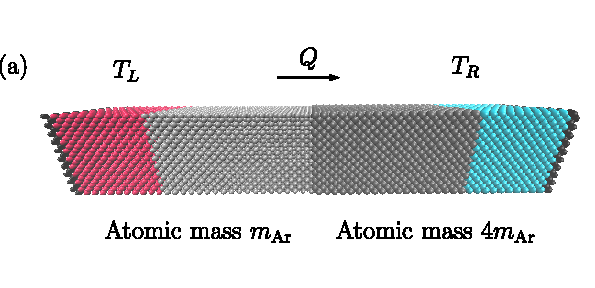
\includegraphics[width=.59\columnwidth]{pics/nemd_fig2a_2.pdf} 
  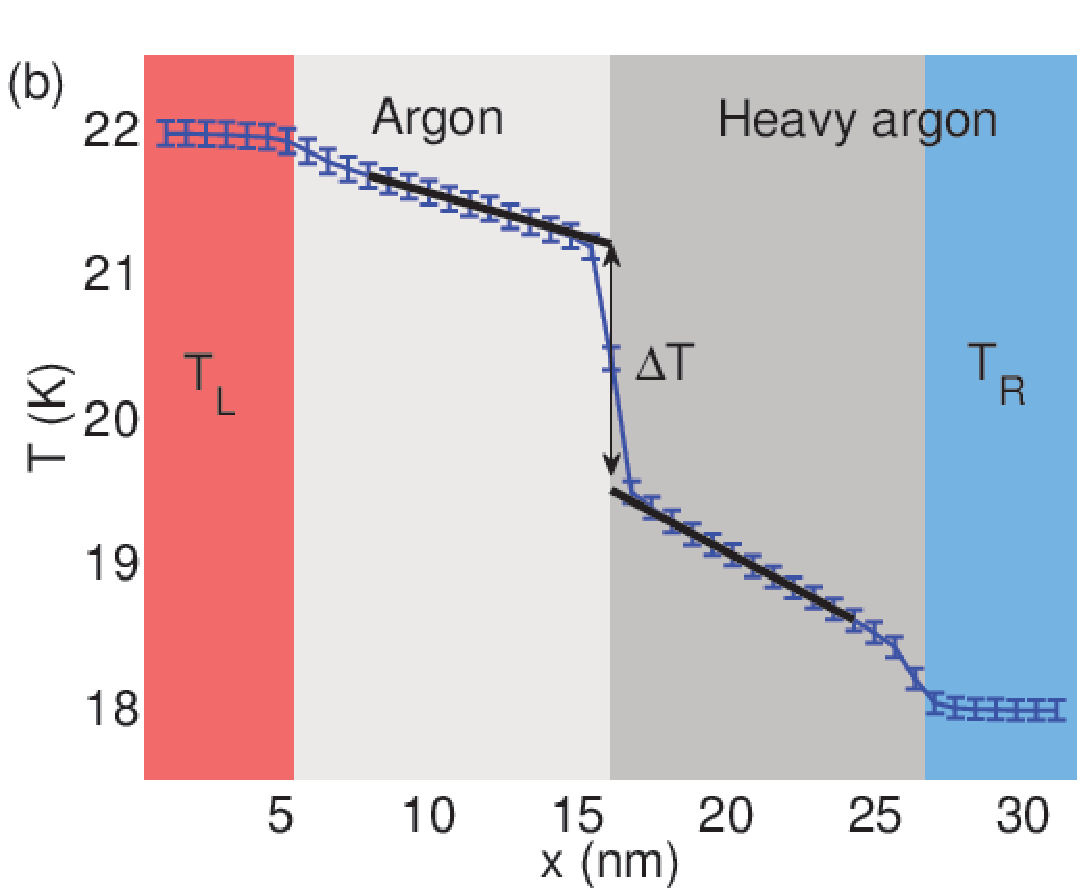
\includegraphics[width=.59\columnwidth]{pics/nemd_fig2b_2.pdf}
  \caption{(a) Simulation geometry used in \citepub{spectral} for investigating the role of anharmonic effects on vibrational energy transfer at mass-mismatched interfaces. (b) Steady-state temperature profile for a specific set of parameters. Reprinted with publisher's permission from \citepub{spectral}.}  
\label{fig:th_spectral_geom}
 \end{center}
\end{figure}

To outline the typical steps involved in a non-equilibrium simulation, consider the example setup of Fig. \ref{fig:th_spectral_geom}(a) used to investigate the anharmonic effects in interfacial heat transfer in \citepub{spectral}. In the setup of Fig. \ref{fig:th_spectral_geom}(a), the whole structure is first allowed to conform to zero-stress state by controlling atomic dynamics using a combination of a Nose-Hoover barostat and thermostat \cite{allentildesley}. Typical equilibration period consists of a few hundreds of thousands of time steps. After the initial equilibration, the size of the simulation box is fixed, and the positions of atoms located at the left- and right-most unit cells are frozen, preventing atomic sublimation at the free surfaces. Particles in the ''hot'' and ''cold'' regions, illustrated by the red and cyan coloured atoms in Fig. \ref{fig:th_spectral_geom}, are coupled to heat baths at temperatures $T_{\textrm{L}}$ and $T_{\textrm{R}}$ by including Langevin or Nos\'e-Hoover terms in their equations of motion. The system is then allowed to reach non-equilibrium steady state by integrating the equations of motion until the kinetic temperature profile shown in Fig. \ref{fig:th_spectral_geom}(b) and the heat current flowing through the system fluctuate around constant values. After this transient period, simulation is continued typically for millions of time steps, and the values of observables such as temperature jump $\Delta T$ at the interface or the heat currents are determined from the trajectories. The statistical error in the determined quantities can be estimated by using standard methods described, e.g., in Ref. \cite{allentildesley}.

LAMMPS simulation package \cite{plimpton95,lammps_website} is used in Publications \cp{spectral}, \cp{cnt} and \cp{twinning} for integrating the equations of motion. The simulations of Publications \cp{fpu} and \cp{fpu2} are carried out using a house-made molecular dynamics code. 

% LAMMPS, house-made code

\iffalse

\subsection{Spectral heat current analysis}
% \subsubsection{Lattice heat current}
\label{sec:spectral}
The main observable of interest in heat transfer simulations is the heat current flowing through system, which can be expressed as a sum of interatomic heat currents flowing across a specified cross-section of the simulation domain. The expression for the interatomic heat current can be determined by calculating the temporal rate of change in the local energy consisting of kinetic and potential energy contributions \cite{hardy63,lepri03}. For the average heat current flowing from atom $j$ to atom $i$ one thereby gets (see \citepub{fpu} for derivation) 
\begin{equation}
 Q_{j\to i} = \left\langle \frac{1}{2} \bb{F}_{ij} \cdot \left( \bb{v}_i+\bb{v}_j \right) \right\rangle, \label{eq:th_Qji}
\end{equation}
where the force acting on atom $i$ due to the interaction with atom $j$ is obtained from the pairwise potential energy $V_{ij}$ as
\begin{equation}
 \bb{F}_{ij} = - \frac{\partial V_{ij}}{\partial \bb{r}_i}.
\end{equation}
The angular brackets in Eq. \eqref{eq:th_Qji} denote non-equilibrium ensemble average, which can be calculated by time-averaging in MD simulations. 

Equation \eqref{eq:th_Qji} cannot directly indicate, which vibrational frequencies are actually responsible for the energy transfer. Such an analysis was enabled in \citepub{spectral}, where an expression for the spectral decomposition $q_{j\to i}(\omega)$ of heat current was derived. The decomposition is defined implicitly through the formula
\begin{equation}
 Q_{j\to i} = \int_0^{\infty} \frac{d\omega}{2\pi} q_{j\to i}(\omega)
\end{equation}
and was shown to be given by the expression
\begin{equation}
 q_{j \to i}(\omega) = 2\textrm{Re} [\tilde K_{ij}(\omega)],
\end{equation}
where $\tilde K_{ij}(\omega)=\int_{-\infty}^{\infty} dt e^{i\omega t}K_{ij}(t)$ is the Fourier transform of the time-domain correlation function
\begin{equation}
 K_{ij}(t_1-t_2) = \frac{1}{2} \left\langle \bb{F}_{ij}(t_1) \cdot \left[ \bb{v}_i(t_2)+\bb{v}_j(t_2)\right] \right\rangle \label{eq:th_Kijt1t2}
\end{equation}
The force-velocity correlation function depends explicitly only on the time-difference $t_1-t_2$ due to the assumed steady-state. 

The correlation function can be calculated by analyzing the force and velocity trajectories obtained from non-equilibrium molecular dynamics simulation. In practice, it is useful expand the interatomic force $\bb{F}_{ij}$ in terms of small displacements from equilibrium positions, allowing for simplifying the post-processing and detailing the relative contributions of linear and non-linear energy transfer mechanisms. The contributions of non-linear terms to the interfacial thermal conductance were analyzed in \citepub{spectral}. In \citepub{cnt}, only the dominant linear term was included in investigating the phonon transmission in carbon nanotubes.

%\label{sec:methods}
\fi


%This section presents the methods used in this thesis to solve the equations of motion presented in Sec. \ref{sec:th_eom} and \ref{sec:th_eom2}. We first discuss the calculation of energy transfer rates from the Green's function methods in Sec. \ref{sec:methods_gf}. While the linearization of the equations excludes detailed modeling of non-linear interactions, it allows for including quantum statistics, full wave properties, and dissipation through effective relaxation rates. The inclusion of dissipation by effective parameters allows for simulating larger systems than when using perturbative approaches such as Keldysh Green's function methods \cite{haugjauho}.  %We also highlight the similarities in the mathematical solution of the Langevin equations and the calculation of observables such as heat currents to appreciate the analogies in phononic, photonic, and electronic transport. 

%After the discussion of Green's function methods, we introduce in Sec. \ref{sec:methods_md} the molecular dynamics (MD) method used for solving the non-linear lattice dynamics equations \eqref{eq:th_eom}. Molecular dynamics simulation is limited to classical statistics, but it automatically accounts for phonon-phonon scattering arising from anharmonic terms in the interatomic potential and is suitable for simulating systems with millions of atoms. As multiple text-books have been written about MD simulations \cite{allentildesley,frenkelsmit}, we only discuss the most important aspects in this section.

% After the brief introduction to MD, we present the calculation of spectral transmission from the Green's function methods in Sec. \ref{sec:methods_gf}. While the linearization of the equations excludes detailed modeling of non-linear interactions, it allows for including quantum statistics, full wave properties, and dissipation through effective relaxation rates. The inclusion of dissipation by effective parameters allows for simulating larger systems than when using perturbative approaches such as Keldysh Green's function methods \cite{haugjauho}. We also highlight the similarities in the mathematical solution of the Langevin equations and the calculation of observables such as heat currents to appreciate the analogies in phononic, photonic, and electronic transport. 


%\subsection{Green's function methods}
%\label{sec:methods_gf}

%This subsection discusses the calculation of observables from the Green's function solution \eqref{eq:th_gf_solution} for the linearized Langevin equations of motion \eqref{eq:th_eom_fourier_phonon}, \eqref{eq:th_eom_fourier_photon}, and \eqref{eq:th_eom_fourier_electron}. The main observable of interest is the heat current flowing to each bath, giving information of the heat flowing in the system and the locally dissipated heat. 

%Calculating the heat current requires solving the equations of motion, which is shown first at a fully general level applicable to any carrier. 

%After the general solution and an example of how the bath current is calculated, we present example geometries considered in this thesis. For phonon and electron transport, the considered geometry is similar to the traditional two-terminal Landauer-B\"uttiker setup \cite{buttiker92,datta} consisting of two leads and a scattering region. Where as the Landauer-B\"uttiker setup is most often used for investigating ballistic quantum transport, the coupling of degrees of freedom to local Langevin baths allows for modeling carrier dissipation. To ensure current conservation, the bath temperatures (and chemical potentials for electrons) must then be solved self-consistently to ensure current conservation. The modeling of dissipative heat transport by Langevin baths is known as self-consistent heat bath model \cite{bolsterli70}. Earlier studies employing the self-consistent heat bath model have, however, only been limited to one-dimensional chains (see, e.g., Refs. \cite{dhar03,dhar06,segal09,bandyopadhyay11}). The self-consistent solution of bath chemical potentials for electrons was, in turn, introduced by B\"uttiker \cite{buttiker86} and d'Amato and Pastawski \cite{damato90}. For electromagnetic energy transfer, such a Langevin model was proposed in \citepub{dipole}.

%\subsubsection{Calculation of observables}

%Before presenting exemplary computation geometries, let us consider the calculation of observables from the linearized Langevin equations, because the procedure is similar for all three different energy transfer mechanisms. As shown in Sec. \ref{sec:th_eom}, the general solution to linear Langevin equation of motion \eqref{eq:th_general} is given by
%\begin{equation}
% \tilde{\bb{x}}(\omega)  = \sum_J \bb{G}(\omega)\tilde \zeta^J(\omega), \label{eq:th_gf_solution2}
%\end{equation}
%where the degrees of freedom collected in the vector variable $\bb{x}$ are either atomic displacements, dipole displacements or electron annihilation operators. The solution \eqref{eq:th_gf_solution2} must be accompanied by the fluctuation-dissipation theorem \eqref{eq:th_xixiom_ohmic_qm} for each bath indexed by the variable $J$, which can be compactly written in terms of the coupling function $\Gamma^J(\omega)=-2\textrm{Im}[\Sigma^J(\omega)]$ as (for atom and dipole displacements)
%\begin{equation}
% \left\langle\tilde \zeta^I(\omega)\tilde \zeta^J(\omega')^T \right\rangle = 2\pi \delta(\omega+\omega') \hbar \Gamma^I(\omega) \left[f_{\textrm{BE}}(\omega,T_J)+ \frac{1}{2} \right] \delta_{IJ} \label{eq:th_zetazeta}
%\end{equation}
%A similar compact FDT holds for electron baths, when the Bose-Einstein function is replaced by the Fermi-Dirac distribution with temperature $T_I$ and chemical potential $\mu_I$.

% With the solution \eqref{eq:th_gf_solution2} and the general FDT \eqref{eq:th_zetazeta}, one can calculate the observables of interest such as local kinetic energy or the locally dissipated power, which reduces to calculating thermal averages of the form $\langle x_i^2 \rangle$ or $\langle x_i\zeta_i \rangle$. The locally dissipated power at atom site $i$, for example, is given by the thermal average of the Langevin force multiplied by the atom velocity, $\langle [m\gamma \dot{\bu}_i-\xi_i]\cdot \dot{\bu}_i \rangle$. Straightforward application of Eq. \eqref{eq:th_gf_solution2} and \eqref{eq:th_zetazeta} gives for $\langle x_i^2\rangle$:
% \begin{alignat}{2}
%   \langle x_i^2 \rangle &= \int_{-\infty}^{\infty}  \int_{-\infty}^{\infty} \frac{d\omega}{2\pi} \frac{d\omega'}{2\pi} \langle \tilde x_i(\omega)x_i(\omega') \rangle \\
%    &= \int_{-\infty}^{\infty}  \int_{-\infty}^{\infty} \frac{d\omega}{2\pi} \frac{d\omega'}{2\pi} \sum_{I,J} \sum_{k,l} G_{ik}(\omega) G_{il}(\omega') \langle \zeta^I_k(\omega) \zeta^J_l(\omega') \rangle \\
%   &= \int_{-\infty}^{\infty}  \frac{d\omega}{2\pi} \sum_{I}  \sum_{k,l} G_{ik}(\omega) G_{il}(-\omega) \hbar \Gamma^I_{kl}(\omega) \left[f_{\textrm{BE}/\textrm{FD}}(\omega,T_I)+ \frac{1}{2} \right]\\
%    &=  \int_{-\infty}^{\infty}  \frac{d\omega}{2\pi} \hbar \sum_I \left[\bb{G}(\omega) \Gamma^I(\omega) \bb{G}(\omega)^{\dagger} \right]_{ii}\left[f_{\textrm{BE}/\textrm{FD}}(\omega,T_I)+ \frac{1}{2} \right].
%  \end{alignat}
% \begin{alignat}{2}
%  \langle \dot{\bu}_i^2 \rangle &= \sum_{\alpha} \int_{-\infty}^{\infty}  \int_{-\infty}^{\infty} \frac{d\omega}{2\pi} \frac{d\omega'}{2\pi} \langle - \omega \omega' \tilde  u_i^{\alpha}(\omega)u_i^{\alpha}(\omega') \rangle \\
%   &= \int_{-\infty}^{\infty}  \int_{-\infty}^{\infty} \frac{d\omega}{2\pi} \frac{d\omega'}{2\pi} (-\omega\omega') \sum_{I,J} G_{ik}^{\alpha\beta}(\omega) G_{jl}^{\alpha\gamma}(\omega') \langle \xi^I_k(\omega) \zeta^J_l(\omega') \rangle \\
%   &= \int_{-\infty}^{\infty}  \frac{d\omega}{2\pi} \sum_{I}G_{ik}(\omega) G_{jl}(-\omega) \hbar \Gamma^I_{kl}(\omega) \left[f_{\textrm{BE}/\textrm{FD}}(\omega,T_I)+ \frac{1}{2} \right]\\
%   &=  \int_{-\infty}^{\infty}  \frac{d\omega}{2\pi} \sum_I \left[\bb{G}(\omega) \Gamma^I(\omega) \bb{G}(\omega)^{\dagger} \right]_{ii}\left[f_{\textrm{BE}/\textrm{FD}}(\omega,T_I)+ \frac{1}{2} \right].
% \end{alignat}
% Following such a procedure, any two-particle correlations can be calculated. As shown in Publications \cp{gf} and \cp{dipole}, calculation of the average heat current $\langle Q^I \rangle$ flowing to bath $I$ leads to the expression \eqref{eq:th_QI}, with the transmission function \eqref{eq:th_caroli}.

% Equation \eqref{eq:th_caroli} is the well-known Caroli form for the transmission function \cite{caroli71}, originally derived for ballistic two-terminal electron transport and later for phonons \cite{mingo06,yamamoto06}. In \citepub{dipole}, Eq. \eqref{eq:th_caroli} was shown to be valid also for electromagnetic energy transfer between a collection of dipoles.

%\subsubsection{Self-consistent heat bath model for vibrational heat transfer}




%where the transmission function between baths $I$ and $J$ is defined as
%\begin{equation}
% \ca{T}_{IJ}(\omega) = \textrm{Tr}\left[\Gamma^I(\omega) \bb{G}(\omega) \Gamma^J(\omega) \bb{G}(\omega)^{\dagger} \right]. \label{eq:th_caroli}
%\end{equation}


\iffalse
\subsubsection{Example for electromagnetic energy transfer}

\begin{figure}
 %\includegraphics[width=15.6cm]{pic1.ps}
%  \includegraphics[width=.49\columnwidth]{../dipole_resubmission/pic1a}
 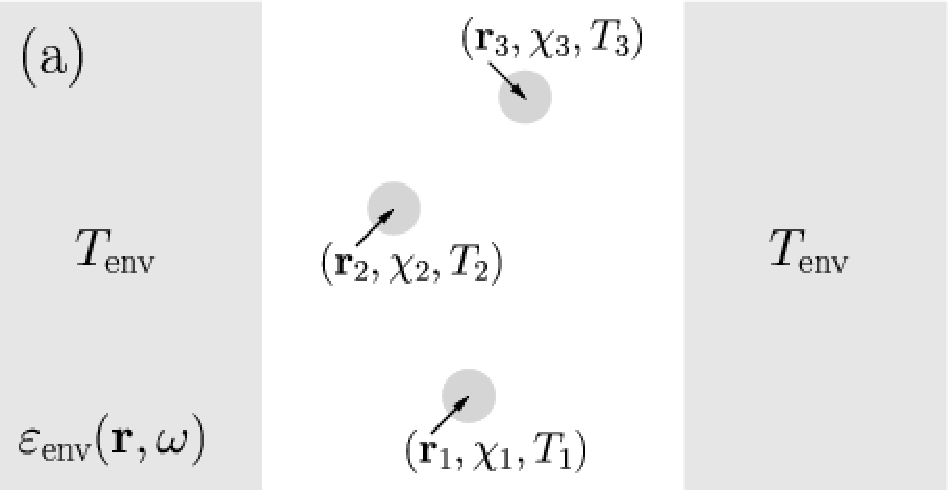
\includegraphics[width=.49\columnwidth]{pics/dipole_pic1a.pdf}
 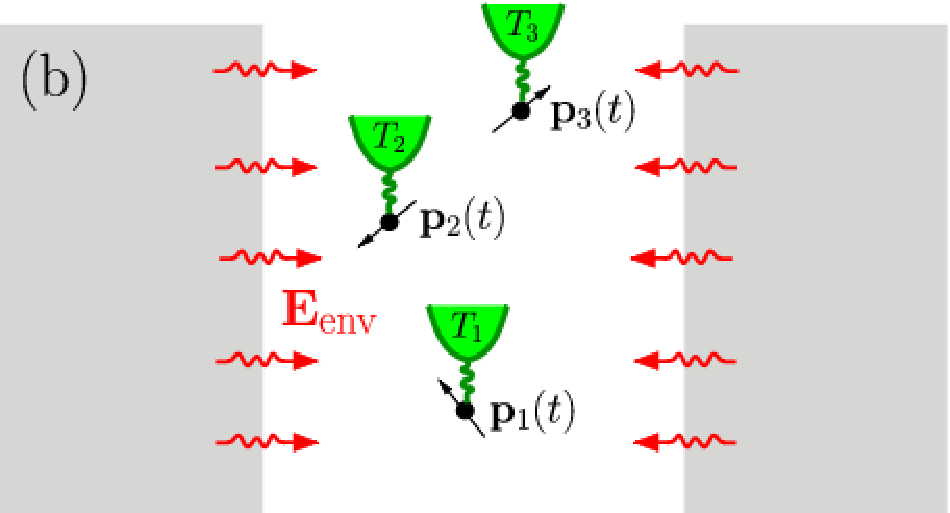
\includegraphics[width=.49\columnwidth]{pics/dipole_pic1b.pdf}
%   \includegraphics[width=.49\columnwidth]{../dipole_resubmission/pic1b}
 \caption{(a) A schematic illustration of an exemplary setup for investigating electromagnetic energy transfer between polar nanoparticles in a microcavity. A collection of dielectric particles with positions $\mathbf{r}_i$, $i\in\{1,\dots,N\}$, electric susceptibilities $\chi_i(\omega)$ and temperatures $T_i$ is located in an inhomogeneous environment, consisting in the shown case of two dielectric (or metallic) bodies forming a cavity. The overall relative permittivity is $\varepsilon(\br,\omega)=\epsenv(\br,\omega)$ outside the particles and $\varepsilon(\br_i,\omega)=1+\chi_i(\omega)$ at the position of each particle coordinate $\br_i$. The two cavity walls, described by the environment dielectric constans, are assumed to act as a source of thermal radiation at temperature $\Tenv$. The polarization field inside each particle $i$ is modeled as an oscillating point dipole moment $\bb{p}_i$ coupled to a local Langevin heat bath at temperature $T_i$ as depicted in (b). The total local field $\bE(\br_i,t)$ driving each dipole moment $\bb{p}_i$ is the sum of the stochastic background field $\bE_{\textrm{env}}(\br_i,t)$ and the fields $\bE_{ij}(t)$ created by each dipole $j$.}%The local bath temperatures $T_i$ correspond to local lattice temperatures, which could either by given fixed temperatures or could be self-consistently determined by the balance of absorption, emission and the in- and outflow of lattice heat. 
\label{fig:gfm_dipole_system}
\end{figure}

We briefly outline the quantum Langevin equation approach to the electromagnetic energy transfer here. The final results for energy transfer rates are equivalent to those calculated from fluctuational electrodynamics \cite{benabdallah11,messina13}, as explained in \citepub{dipole}. 

An exemplary system is depicted in Fig. \ref{fig:gfm_dipole_system}. Dielectric particles with positions $\mathbf{r}_i$, $i\in\{1,\dots,N\}$ are located in an inhomogeneous environment characterized by the environment's dielectric constant $\epsenv(\br,\omega)$. Inhomogeneous $\epsenv(\br,\omega)$ acts as a source of non-blackbody thermal radiation (at temperature $\Tenv$) and also scatters the radiation emitted by the particles, thereby modifying the dipole-dipole energy transfer rates compared to the free space. The overall relative permittivity is given by $\varepsilon(\br_i,\omega)=1+\chi_i(\omega)$ at the locations of the particles ($\chi_i$ being the electric susceptibility of particle $i$) and $\varepsilon(\br,\omega)=\epsenv(\bb{r},\omega)$ elsewhere. 

% The microscopic dipole moments, which represent the fluctuating electric polarization inside each particle, are coupled to (1) local heat baths describing thermal fluctuations and dissipation, (2) to the electromagnetic field arising from other dipoles, and (3) to the thermal field originating from the environment. Following the dipole approximation \cite{novotny}, we assume each particle to be smaller than the optical wavelength so that we can treat the particles as dipoles located at locations $\br_i$, but the theory can be straightforwardly generalized to larger particles as well by dividing the particles into small dipolar volumes as in the traditional discrete dipole method \cite{novotny}. 

In the oscillating dipole model \cite{rosa10,rosa11}, the local dynamics of each dipole is modeled by the classical oscillator model accompanied by quantum Langevin dynamics. The equation of motion for the local dipole displacement $\bd_i$ is then given by Eq. \eqref{eq:th_eom2}. In a fully optical treatment, the microscopic oscillator parameters (mass $m$, charge $q$, and damping coefficient $\gamma$) can be related to the electric susceptibilities of the particles as explained in Refs. \cite{rosa10,rosa11}. Solving the Fourier-transformed linear system of equations \eqref{eq:th_eom_fourier_photon} gives
\begin{equation}
 \tilde{\bd}(\omega) = -\bb{G}(\omega) \left[\tilde{\xi}(\omega)+q\Eenvtilde(\omega) \right], \label{eq:th_bd_sol}
\end{equation}
where $\bb{G}(\omega)$ is the (negative) inverse of the coefficient matrix multiplying the dipole displacements $\bd_i$ in Eq. \eqref{eq:th_eom_fourier_photon}.

With the solution \eqref{eq:th_bd_sol}, one can proceed to calculating energy transfer rates at each dipole. The heat transfer rates between particles could in general be calculated from the electromagnetic Poynting vector, but the calculations can be simplified by energy conservation arguments. A direct calculation shows that the expectation value of the Poynting vector's flux across a surface $\partial V_i$ enclosing a particle $i$, equal to the power of the emitted radiation field, satisfies (see \citepub{dipole})
\begin{equation}
 \left\langle \int_{\partial V_i} \bb{S} \cdot d\bb{S} \right\rangle = - \langle Q_i \rangle,
\end{equation}
where the energy current to the bath is given by the bath force multiplied by the dipole moment ''velocity'': $Q_i = (m\gamma \dot{\bd}_i-\xi_i)\cdot \dot{\bd}_i$. Therefore, $\langle Q_i\rangle$ can be interpreted as the locally absorbed power. Direct calculation carried out in \citepub{dipole} shows that 
\begin{alignat}{2}
 \langle Q_i \rangle &= \int_0^{\infty}\frac{d\omega}{2\pi} \hbar\omega \sum_{j} \ca{T}_{ij}(\omega) \left[f_B(\omega,T_j)-f_B(\omega,T_i ) \right] \notag \\
  & \quad + \int_0^{\infty} \frac{d\omega}{2\pi} \hbar \omega \ca{T}_{i,\textrm{rad}}(\omega)\left[ f_B(\omega,\Tenv)-f_B(\omega,T_i)\right].
\end{alignat}
Here the dipole-dipole transmission function is defined as
\begin{equation}
 \ca{T}_{ij}(\omega) = \textrm{Tr} \left[\Gamma_i(\omega) \bb{G}(\omega) \Gamma_j(\omega) \bb{G}(\omega)^{\dagger} \right]
\end{equation}
and the dipole-environment transmission is 
\begin{equation}
 \ca{T}_{i,\textrm{rad}}(\omega) =  \textrm{Tr} \left\{ \Gamma_i(\omega) \left[ \bb{G}(\omega) \Gamma_{\textrm{rad}}(\omega) \bb{G}(\omega)^{\dagger} \right]_{ii} \right\}, \label{eq:th_Tirad}
\end{equation}
where $\Gamma_i(\omega)=2m\gamma \omega \unitdyadic$ for the dipoles and $\Gamma^{\textrm{rad}}_{ij}(\omega)= 2 q^2\omega^2\mu_0 \textrm{Im}[\gem(\br_i,\br_j;\omega)]$ is the coupling function to the background radiation field.

To calculate the transmission functions, it is useful to express the transmission function in terms of purely optical quantities. This can be achieved by (i) absorbing the microscopic, auxiliary parameters $m$, $q$, $\gamma_i$ to the definitions of the local polarizabilities and (ii) expressing the Green's function in terms of the electromagnetic Green's dyadics. As shown in \citepub{dipole}, the dipole-dipole energy transmission function can be written in terms of the Clausius-Mossotti polarizabilities
\begin{equation}
\alpha_{\textrm{CM}}^i(\omega) = 3\Delta V_i \frac{\varepsilon_i(\omega)-1}{\varepsilon_i(\omega)+2} \unitdyadic. \label{eq:gfm_alphacm_epsilon}
\end{equation}
of the particles as
\begin{equation}
   \ca{T}_{ij}(\omega) = 4 \kw^4 \textrm{Tr} \left[ \textrm{Im}[\alpha^i_{\textrm{CM}}(\omega)] \gemfull_{ij}\pom \textrm{Im}[\alpha^j_{\textrm{CM}}(\omega)] \gemfull_{ji}(\omega)^{\dagger}\right]. \label{eq:tij_final}
\end{equation}
Here the electromagnetic Green's dyadic $\gemfull(\omega)$ expressed in terms of the Clausius-Mossotti polarizabilities of the particles has been defined as 
\begin{alignat}{2}
 \gemfull(\omega) &= \frac{1}{\kw^2} \left[\frac{1}{1-\kw^2 \gem(\omega)\alpha_{\textrm{CM}}(\omega)}\right] \alpha_{\textrm{CM}}(\omega)^{-1} \\
  &\equiv \frac{1}{\kw^2} \alpha_{\textrm{CM}}(\omega)^{-1} + \underbrace{ \left[\frac{1}{1-\kw^2 \gem(\omega)\alpha_{\textrm{CM}}(\omega)} \right] \gem(\omega)}_{\tildegemfull}. \label{eq:gfm_gemmb_cm_app}
\end{alignat}
The first term of Eq. \eqref{eq:gfm_gemmb_cm_app} is local and does not contribute to dipole-dipole energy transfer. The second term of Eq. \eqref{eq:gfm_gemmb_cm_app}, denoted by $\tildegemfull$, is non-local and therefore responsible for dipole-dipole energy transfer. By comparing the expression \eqref{eq:gfm_gemmb_cm_app} to the one obtained from FED \cite{benabdallah11}, one can show that $\tildegemfull$ is readily interpreted as the electromagnetic Green's dyadic that fully incorporates the scattering caused by the dipoles.

\fi

%\subsubsection{Electrons}

%\subsubsection{Photons}

% \subsubsection{Coupling of models}

% \subsection{Molecular dynamics}
% \label{sec:methods_md}
% 
% \subsubsection{Background}
% 
% Molecular dynamics simulations are a powerful tool for modeling the vibrational energy transfer in atomic scale systems. In MD, the classical Newton's equations of motion \eqref{eq:th_eom}  are integrated numerically. The forces $\bb{F}_i$ are calculated from an analytical expression obtained from the interatomic potential function $\ca{V}$ as $\bb{F}=-\partial \ca{V}/\partial \bb{r}_i$ and they therefore include all orders of anharmonic terms. Langevin forces satisfying the classical FED \eqref{eq:th_xixiom_ohmic_classical} act as heat sources and sinks enabling energy transfer and are included for only a small subset of atoms.  By simulating the steady-state non-equilibrium for sufficiently long times, one can extract values of macroscopic observables such as the heat current accurately by time-averaging. Based on the ergodicity principle, the time averages are expected to equal the statistical average over the corresponding ensemble. In the following, we briefly go through the most important aspects related to a MD simulation.
% 
% % One key aspect of the method is the assumption of ergodicity: statistical ensemble average can be calculated from a time average, meaning that  %In a microcanonical simulation, for example, the system should sample all the states that lie on the constant-energy manifold determined by the initial conditions. 
% 
% In MD, the equations of motion are integrated numerically using a finite-difference method. The pool of the finite-difference methods includes, e.g., Euler methods, Verlet methods, Runge-Kutta methods, the leap-frog method and predictor-corrector methods \cite{allentildesley}. In all the simulations of this work, the velocity Verlet algorithm was employed to integrate the equations of motion. While velocity Verlet exhibits moderate short-term energy drift, it is very simple to implement, efficient and it possesses very small long-term energy drift due to its being both time-reversible and symplectic \cite{frenkelsmit}. The velocity Verlet update equations for the positions $\bb{r}_i$ and velocities $\bb{v}_i=\dot{\bb{r}}_i$ are \cite{allentildesley}
% \begin{alignat}{2}
%   \bb{r}_i(t+\Delta t) &= \bb{r}_i(t) + \bb{v}_i(t)\Delta t+  \frac{1}{2}\bb{a}_i(t) \Delta t^2 + \mathrm{O}(\Delta t^4) \\
%   \bb{v}_i(t+\Delta t) &= \bb{v}_i(t) + \frac{ \bb{a}_i(t)+\bb{a}_i(t+\Delta t)}{2} \Delta t+ \mathrm{O}(\Delta t^2) ,
% \end{alignat}
% where $\Delta t$ is the time step and $\bb{a}_i(t)=\bb{F}_i(t)/m_i$ is the acceleration.
% 
% \begin{figure}[tb]
%  \begin{center}
%   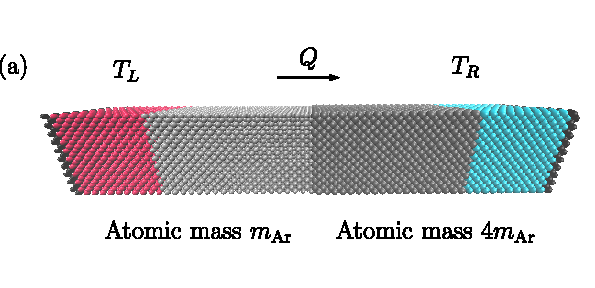
\includegraphics[width=.59\columnwidth]{pics/nemd_fig2a_2.pdf} 
%   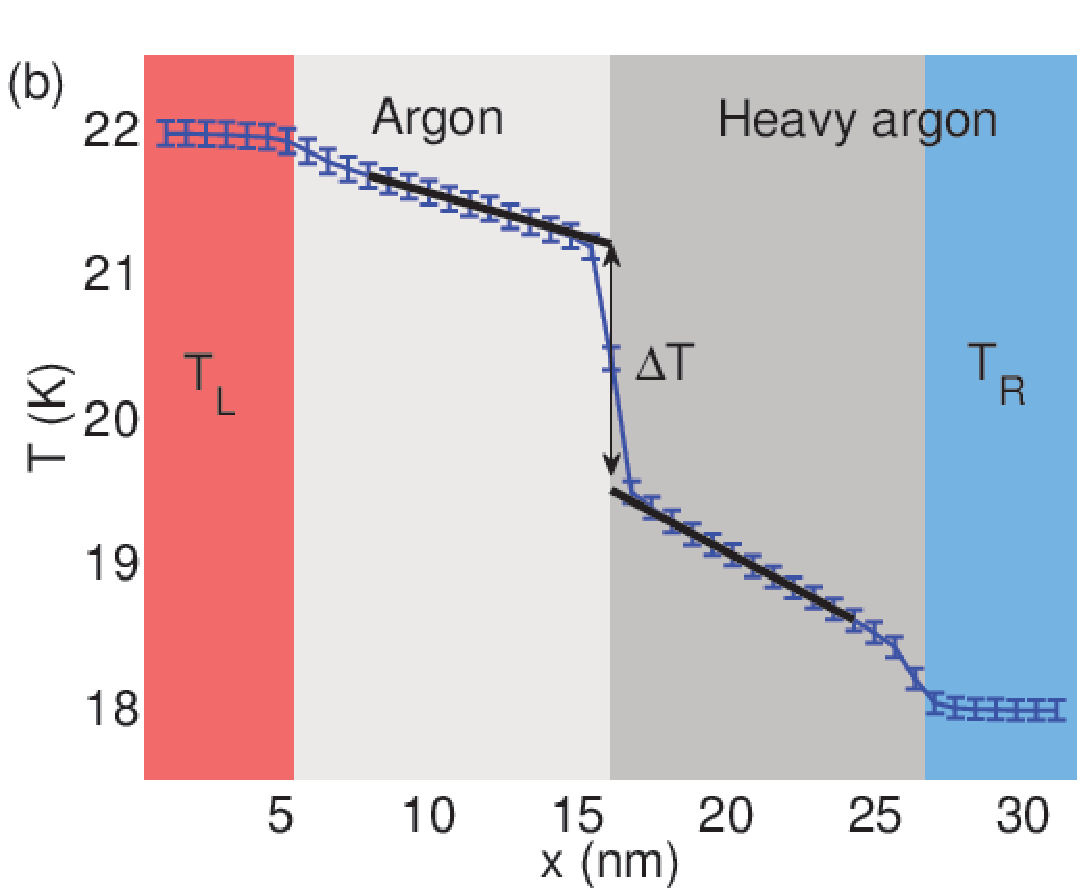
\includegraphics[width=.59\columnwidth]{pics/nemd_fig2b_2.pdf}
%   \caption{(a) Simulation geometry used in \citepub{spectral} for investigating the role of anharmonic effects on vibrational energy transfer at mass-mismatched interfaces. (b) Steady-state temperature profile for a specific set of parameters. For details, see \citepub{spectral}.}  
% \label{fig:th_spectral_geom}
%  \end{center}
% \end{figure}
% 
% 
% To outline the typical steps involved in a non-equilibrium simulation, consider the example setup of Fig. \ref{fig:th_spectral_geom}(a) used to investigate the anharmonic effects in interfacial heat transfer in \citepub{spectral}. First the whole structure is equilibrated by running a zero-pressure simulation at prescribed temperature using a combination of a Nose-Hoover barostat and thermostat, allowing the structure to conform to zero-stress state. Typical equilibration period consists of a few hundreds of thousands of time steps. After the initial equilibration, the size of the simulation box is fixed, as are atoms located at the left- and right-most unit cells in the system. This prevents atomic sublimation at the free surfaces. Particles in the ''hot'' and ''cold'' regions, illustrated by the red and cyan coloured atoms in Fig. \ref{fig:th_spectral_geom}, are coupled to heat baths at temperatures $T_{\textrm{L}}$ and $T_{\textrm{R}}$. The system is then allowed to reach non-equilibrium steady state by running MD until the temperature profile shown in Fig. \ref{fig:th_spectral_geom}(b) and the heat current flowing through the system fluctuate around constant values. After this initial period, simulation is continued typically for millions of time steps, and the values of the observables of interest are collected from the run. The statistical error in the collected observables can be estimated by using standard methods described, e.g., in \cite{allentildesley}.

% LAMMPS, house-made code

% \subsubsection{Spectral heat current analysis}
% % \subsubsection{Lattice heat current}
% \label{sec:spectral}
% The main observable of interest in heat transfer simulations is the heat current flowing through system, which can be expressed as a sum of interatomic heat currents flowing across a specified cross-section of the simulation domain. The expression for the interatomic heat current can be determined by calculating the temporal rate of change in the local energy consisting of kinetic and potential energy contributions \cite{hardy63,lepri03}. For the average heat current flowing from atom $j$ to atom $i$ one thereby gets (see \citepub{fpu} for derivation) 
% \begin{equation}
%  Q_{j\to i} = \left\langle \frac{1}{2} \bb{F}_{ij} \cdot \left( \bb{v}_i+\bb{v}_j \right) \right\rangle, \label{eq:th_Qji}
% \end{equation}
% where the force acting on atom $i$ due to the interaction with atom $j$ is obtained from the pairwise potential energy $V_{ij}$ as
% \begin{equation}
%  \bb{F}_{ij} = - \frac{\partial V_{ij}}{\partial \bb{r}_i}.
% \end{equation}
% The angular brackets in Eq. \eqref{eq:th_Qji} denote non-equilibrium ensemble average, which can be calculated by time-averaging in MD simulations. 
% 
% Equation \eqref{eq:th_Qji} cannot directly indicate, which vibrational frequencies are actually responsible for the energy transfer. Such an analysis was enabled in \citepub{spectral}, where an expression for the spectral decomposition $q_{j\to i}(\omega)$ of heat current was derived. The decomposition is defined implicitly through the formula
% \begin{equation}
%  Q_{j\to i} = \int_0^{\infty} \frac{d\omega}{2\pi} q_{j\to i}(\omega)
% \end{equation}
% and was shown to be given by the expression
% \begin{equation}
%  q_{j \to i}(\omega) = 2\textrm{Re} [\tilde K_{ij}(\omega)],
% \end{equation}
% where $\tilde K_{ij}(\omega)=\int_{-\infty}^{\infty} dt e^{i\omega t}K_{ij}(t)$ is the Fourier transform of the time-domain correlation function
% \begin{equation}
%  K_{ij}(t_1-t_2) = \frac{1}{2} \left\langle \bb{F}_{ij}(t_1) \cdot \left[ \bb{v}_i(t_2)+\bb{v}_j(t_2)\right] \right\rangle \label{eq:th_Kijt1t2}
% \end{equation}
% The force-velocity correlation function depends explicitly only on the time-difference $t_1-t_2$ due to the assumed steady-state. 
% 
% The correlation function can be calculated by analyzing the force and velocity trajectories obtained from non-equilibrium molecular dynamics simulation. In practice, it is useful expand the interatomic force $\bb{F}_{ij}$ in terms of small displacements from equilibrium positions, allowing for simplifying the post-processing and detailing the relative contributions of linear and non-linear energy transfer mechanisms. The contributions of non-linear terms to the interfacial thermal conductance were analyzed in \citepub{spectral}. In \citepub{cnt}, only the dominant linear term was included in investigating the phonon transmission in carbon nanotubes.


%This chapter is devoted to the microscopic theory of energy transfer. In Sec. \ref{sec:th_vibtheory}, the theoretical description of atomic vibrations in a lattice is described. 

% In the publications included in this thesis, we have employed molecular dynamics (MD) simulations and Green's function (GF) calculations to model vibrational heat transfer in nanostructures. It is common to both of these methods that one needs to choose how to describe interatomic interactions and the coupling to external heat baths. Before describing MD and GF calculations in Secs. \ref{sec:md} and \ref{sec:gf}, we therefore briefly review the chosen interatomic potentials and the theory of Langevin heat baths below in Secs. \ref{sec:th_interatomicpotential} and \ref{sec:th_langevin}. When discussing the MD method, we also present the recently developed expression for the spectral heat current distribution.

% For electromagnetic energy transfer, we have employed the same Langevin theory as in vibrational heat transfer to describe the microscopic dipolar thermal fluctuations. This theory is presented in Sec. \ref{sec:em_methods}

\iffalse

\section{Vibrational heat transfer}
\label{sec:th_vibtheory}

This section details the theory of vibrational heat transfer in nanoscale. We start in Subsection \ref{sec:th_phonons} by defining the lattice Hamiltonian and define phonons. Various models for interatomic potential energy used in this thesis are listed in Subsection \ref{sec:th_interatomicpotential}. Langevin theory, which is used in all but one publication of this thesis for the theoretical description of thermalization, is detailed in Subsection \ref{sec:th_langevin}.

\subsection{Lattice Hamiltonian and phonons}
\label{sec:th_phonons}
%As discussed in Chap. 1, propagating lattice vibrations carry heat in crystalline solids, and the quanta of such propagating vibrations are called phonons. The theoretical description is based essentially on the equations of motion for the atoms in the solid. Because fully quantum description does not easily allow for accounting for non-linear dynamics, which play an essential role in any system with non-negligible phonon-phonon interactions, the discussion below treats the atomic dynamics classically. 

%\begin{itemize}
% \item The goals of this work
%\end{itemize}
The theoretical description of lattice heat transfer is based on the dynamical equations of motion for the atoms constituting the lattice. The equations of motion are generally dictated by the Hamiltonian \cite{ziman}
\begin{equation}
 \ca{H} = \sum_{i=1}^N \frac{\bb{p}_i^2}{2m_i} + \ca{V}(\bb{r}_1,\dots,\bb{r}_N). \label{eq:th_hamiltonian}
\end{equation}
Here $\br_i$, $\bp_i$, and $m_i$ are the position, momentum and mass of atom $i$, respectively. The total number of atoms (which can also be infinite) is denoted by $N$. The first term of Eq. \eqref{eq:th_hamiltonian} is the total kinetic energy of the atoms and the second term $\ca{V}$ is the interatomic potential energy responsible for the interatomic interactions. The choice of the potential energy function $\ca{V}$ is crucial for an accurate description of the lattice dynamics and, consequently, of energy transfer. Models for $\ca{V}$ used in this work are explained in detail bwlow in Subsection \ref{sec:th_interatomicpotential}.

Applying Hamilton's equations of motion $\dot{\br}_i=\partial H/\partial \bp_i$ and $\dot{\bp}_i=-\partial \ca{H}/\partial \br_i$ \cite{fetter} gives Newton's law
\begin{equation}
 m_i \ddot{\br}_i = \bb{F}_i, \label{eq:th_eom}
\end{equation}
where the force acting on atom $i$ is
\begin{equation}
 \bb{F}_i = - \frac{\partial \ca{V}}{\partial \bb{r}_i}. \label{eq:th_force}
\end{equation}
For given initial conditions $\br_i(0)$ and $\dot{\br}_i(0)$, Eq. \eqref{eq:th_eom} determines the time evolution of atomic trajectories. To model energy transfer, the equations of motion are supplemented by terms accounting for coupling to external heat baths. In this work, we mostly employ Langevin heat baths that turn the equations of motion into stochastic equations and ensure that the long-term atomic trajectories correctly sample the non-equilibrium statistical ensemble. Langevin theory is presented in Sec. \ref{sec:th_langevin}.

Equation \eqref{eq:th_eom} generally describes the motions of atoms and molecules in solid, gas, and liquid systems. In solids, the atoms vibrate close to their equilibrium positions $\br_i^0$ and one can gain more insight into the lattice dynamics by only considering small displacements from the equilibrium. The positions $\br_i^0$ are defined by the condition of zero force:
\begin{equation}
 \left. \frac{\partial \ca{V}}{\partial \br_i} \right|_{\br_j=\br_j^0 \quad \forall j} = 0. \label{eq:th_zeroforce}
\end{equation}
Assuming that the atoms remain close to the equilibrium positions, one can expand the potential energy in Taylor series in terms of the displacements $\bu_i=\br_i-\br_i^0$:
\begin{equation}
 \ca{V} = \ca{V}_0 + \frac{1}{2} \sum_{i,j} \sum_{\alpha,\beta} u_i^{\alpha} K_{ij}^{\alpha \beta} u_j^{\beta}  + \ca{O}(u^3). \label{eq:th_V_taylor}
\end{equation}
Here the Cartesian coordinate directions $\alpha,\beta \in \{x,y,z\}$ have been written explicitly for clarity and the second-order term is proportional to the ''force constant''
\begin{equation}
 K_{ij}^{\alpha\beta} = \left. \frac{\partial^2 \ca{V}}{\partial u_i^{\alpha} \partial u_j^{\beta}} \right|_{\bu=\mathbf{0}}. \label{eq:th_K_def}
\end{equation}
The first-order derivative term in \eqref{eq:th_V_taylor} vanished based on Eq. \eqref{eq:th_zeroforce} and the last term is of third order in displacements.

In the case that the third-order term can be neglected, employing Eq. \eqref{eq:th_V_taylor} in the equation of motion \eqref{eq:th_eom} gives the system of linear equations
\begin{equation}
 m_i \ddot{u}_i^{\alpha} = - \sum_j \sum_{\beta} K_{ij}^{\alpha\beta} u_j^{\beta}.
\end{equation}
Following standard eigenmode theory \cite{fetter}, the eigenmodes of the system can be found by diagonalizing the matrix $D_{ij}^{\alpha\beta} = (m_i\omega^2 \delta_{ij}\delta
^{\alpha\beta}-K_{ij}^{\alpha\beta})$. In a periodically repeating crystal, the eigenmodes can be labeled by the wavevectors $\bb{q}$ belonging to the first Brillouin zone \cite{ziman} and the branch $p \in \{1,\dots,3N_{\textrm{cell}}\}$, where $N_{\textrm{cell}}$ is the number of atoms in the unit cell. The eigenmodes are called phonon modes, while phonons are the discrete quanta of eigenmode occupation. The eigenfrequencies $\omega(\bb{q},p)$ form the phonon bandstructure, specifying the relation between the wavevectors and frequencies supporting propagating phonon modes. As an example, Fig. \ref{fig:th_nika} shows the phonon bandstructure of graphene, a single monolayer of graphite.

\begin{figure}
\begin{center}
 \includegraphics[width=8.6cm]{pics/nika09_fig3.pdf}
 \caption{Phonon bandstructure of graphene, calculated using the valence force field method \cite{nika09}. The two-dimensional bandstructure is plotted along one-dimensional lines between special points in graphene reciprocal lattice, denoted by $\Gamma$, $M$ and $K$. Because graphene has two atoms per unit cell, there are altogether six phonon branches. The three branches that have vanishing frequencies at the $\Gamma$ point are called longitudinal acoustic (LA), transverse acoustic (TA) and out-of-plane acoustic (ZA). The optical modes LO, TO and ZO are labeled similarly. Reprinted with permission from Ref. \cite{nika09}.}
\label{fig:th_nika}
\end{center}
\end{figure} 

When the anharmonic part in Eq. \eqref{eq:th_V_taylor} is neglected, the phonon eigenmodes are exact eigenmodes of the system and cannot dissipate their energy, giving rise to infinite thermal conductivity \cite{ziman}. The anharmonic terms give rise to phonon-phonon scattering \cite{ziman}, which is the primary phonon decay mechanism in crystalline solids at high temperatures. In Publications \cp{fpu}, \cp{fpu2}, \cp{spectral}, \cp{cnt}, and \cp{twinning}, we have employed classical molecular dynamics simulations fully accounting for anharmonic scattering. In \citepub{gf}, anharmonic effects are mimicked by the self-consistent heat bath model \cite{bolsterli70}, allowing for the inclusion of quantum statistics as well. These methods are explained in more detail below in Chap. XXX.

\subsection{Models for interatomic potential energy}
\label{sec:th_interatomicpotential}

%Typically, the analytical form of the interatomic potential is inferred from quantum-mechanical calculation and the free parameters are fitted to reproduce experimentally known quantities such as the lattice constant, bulk modulus, atomization energy, and so on. For this reason, the interatomic potentials are often called semi-empirical. In chemistry, the term force field is used instead of interatomic potential.

As mentioned in Sec. \ref{sec:intro_vibtheory}, a crucial physical aspect of correctly describing the lattice dynamics and, therefore, vibrational energy transfer is the choice of interatomic potential energy function $\ca{V}$. In general, the interatomic potential consists of pair potential terms and many-body terms. 
%, which we assume to only consist of the three-body terms $V^{(3)}(\bb{r}_i,\bb{r}_j,\bb{r}_k)$:
%\begin{equation}
% U(\bb{x}) = \frac{1}{2}  \sum_{ i,j } V^{(2)}(|\bb{r}_{i}-\bb{r}_j|) + \frac{1}{6} \sum_{i,j,k} V^{(3)}(\bb{r}_i,\bb{r}_j,\bb{r}_k)
%\end{equation}
A very simple example of a pure pair-potential is the Fermi-Pasta-Ulam (FPU) potential used by Fermi, Pasta, and Ulam to investigate the minimal necessary conditions for thermalization in one-dimensional system. In the FPU model, atoms with displacement $u_i$ from the equilibrium position are assumed to be connected to their nearest neighbors by anharmonic springs with the pair-wise energy of the form
\begin{equation}
  V_{ij}^{\textrm{FPU}} = \frac{1}{2} k (u_i-u_j)^2 + \frac{\alpha}{3} (u_i-u_j)^3+ \frac{\beta}{4} (u_i-u_j)^4, \label{eq:th_fpu}
\end{equation}
which is referred to as the FPU potential. The FPU potential can be considered to arise from the Taylor expansion of a more realistic potential (such as LJ). The models for $\beta=0$ and $\alpha=0$ are known as $\alpha$-FPU and $\beta$-FPU, respectively, and both have been employed extensively in investigating thermalization and thermal conduction in low-dimensional systems \cite{}. In Publications \cp{fpu} and \cp{fpu2}, the $\beta$-FPU potential was used to model the anharmonic interactions in a square lattice. In Publication \cp{gf}, the anharmonic interactions were mimicked by the coupling to self-consistent heat baths (see Sec. \ref{sec:gf}), and only the harmonic term of Eq. \eqref{eq:th_fpu} was included ($\alpha=\beta=0$).

Another very common pair-potential is the Lennard-Jones (LJ) potential \cite{allentildesley}
\begin{equation}
 V_{ij}^{\textrm{LJ}}(r_{ij}) = 4\varepsilon \left[\left( \frac{\sigma}{r_{ij}}\right)^{12}-\left( \frac{\sigma}{r_{ij}}\right)^6  \right],
\end{equation}
where $\varepsilon$ is the interaction energy, $\sigma$ determines the equilibrium distance $r_0$ of atoms ($r_0=2^{1/6}\sigma$ for two particles), and $r_{ij}$ is the interparticle distance. The repulsive term $(\sigma/r_{ij})^{12}$ models the strong atomic repulsion at short distances, arising from the overlapping of electron clouds. The attractive term $-(\sigma/r_{ij})^{6}$ accounts for the weak van der Waals attraction at large distances, arising from the interaction of the fluctuating dipole moments due to, e.g., electron polarization. The LJ potential accurately describes interatomic interactions between noble gas atoms such as argon and, thanks to its simple form, it is also often used to investigate the qualitative features of heat transfer in solids \cite{}. The LJ potential was used in Publication \cp{spectral} to model the interatomic interactions in investigating the spectral conductance between mass-mismatched solids arranged in a face-centered cubic lattice. %Because the LJ interaction does not account for the local environment, however, the LJ potential cannot describe, e.g., covalent bonding. %It is used a constituent in more complicated potentials to describe the van der Waals attractions. Due to its simple form, it is also often used 


Pure pair-potentials such as the Lennard-Jones potential cannot describe, e.g., covalent bonding, where the strength of local bonding is strongly influenced by the environment. Therefore, a more sophisticated potential is needed to model, for example, carbon materials. A typical example of a many-body potential is the Tersoff potential \cite{tersoff88b}
\begin{equation}
 V_{ij}(r_{ij}) = f_C(r_{ij}) \left[A e^{-\lambda_1 r_{ij}} - B b_{ij} e^{-\lambda_2 r_{ij}}) \right],
\end{equation}
where the taper function 
\begin{equation}
 f_C ( r) = \left\{ \begin{array}{ll}
                     1 & \textrm{for } r<R-D,\\
		     \frac{1}{2}-\frac{1}{2}\sin\left(\frac{\pi}{2}\frac{r-R}{D} \right) & \textrm{for } R-D < r < R+D, \\
		     0 & \textrm{for } r>R+D
                    \end{array}
 \right.
\end{equation}
gradually turns off the pair-wise interaction between $r_{ij}=R-D$ and $r_{ij}=R+D$. The strength of interatomic attraction is controlled by the coefficient
\begin{equation}
 b_{ij} = \left( 1+\beta^n \zeta_{ij}^n \right)^{-1/(2n)},
\end{equation}
where the dependence on the local environment appears in the definition 
\begin{equation}
 \zeta_{ij} = \sum_{k\neq i,j} f_C(r_{ik}) g(\Theta_{ijk}) \exp\left[\lambda_3^3(r_{ij}-r_{ik})^3 \right] .
\end{equation}
Here $\Theta_{ijk}$ is the angle between bonds $ij$ and $ik$. The angle function is defined as 
\begin{equation}
 g(\Theta) = 1 + \frac{c^2}{d^2} - \frac{c^2}{d^2 + (\cos \Theta-\cos \Theta_0)^2}
\end{equation}
The parameters $R$, $D$, $A$, $\lambda_1$, $B$, $\lambda_2$, $\beta$, $n$, $\lambda_3$, $c$, $d$, and $\Theta_0$ depend on the material under study. The Tersoff parameters for carbon systems were originally fit to the experimentally known cohesive energies of various carbon systems and the lattice constant and bulk modulus of diamond \cite{tersoff88a}. Recently, Lindsay and Broido \cite{lindsay10} suggested an improved set of parameters found by giving more weight to matching the experimentally measured phonon dispersion for graphite. This optimized Tersoff potential was used in Publication \cp{cnt} for carbon nanotubes. In \citepub{twinning}, many-body Stillinger-Weber potential \cite{stillinger85} was used to model interactions between Si atoms constituting Si nanowire. 


\subsection{Langevin theory} 
\label{sec:th_langevin}
The equations of motion \eqref{eq:th_eom} only describe the interactions between the constituents of the system under study. To enable steady-state energy transfer, some of the degrees of freedom must be coupled to external heat baths acting as heat sources and sinks. Because Langevin heat baths are employed in all but one publication included in this thesis, we briefly review the Langevin theory.

In Langevin theory, the particle coupled to the bath is imagined to interact with a collection of harmonic oscillators at a prescribed temperature. The bath degrees of freedom are ''integrated out'' so that their interaction with the system under study is described effectively by the Langevin forces \cite{weiss}. The general Langevin equation obtained through such a procedure reads \cite{dhar06}
\begin{equation}
 m\ddot{\bu}_i(t) =  \bb{F}_i(t) - \int_{0}^{\infty}dt' \Sigma_i(t') \bb{u}_i(t-t') + \xi_i(t), \label{eq:th_eom_langevin}
\end{equation}
where, for the simplicity of discussion, we assume that the baths are spatially uncorrelated so that the bath self-energy $\Sigma_i$ is spatially local. The self-energy describes the dynamical interactions and damping induced by the coupling to the heat bath oscillators. The force $\bb{F}_i$ is due to interactions with particles not in the reservoir and the auto-correlation function of the random force $\xi_i$ is related to the damping self-energy $\Sigma_i(t)$ and bath temperature $T_i$ through the fluctuation-dissipation theorem (FDT) \cite{dhar06}
\begin{equation}
 \langle \xi_i(t)\xi_i(t') ^T\rangle = \int_{-\infty}^{\infty} \frac{d\omega}{2\pi} e^{-i\omega(t-t')} \hbar \Gamma_i(\omega) \left[f_B(\omega,T_i)+\frac{1}{2}\right] \bb{I}_{3\times3}. \label{eq:th_xixit}
\end{equation}
Here $\Gamma_i(\omega)=-2\textrm{Im}[\Sigma_i(\omega)]$ is called the bath coupling function \cite{dhar06}. The quantum statistics appear through the Bose-Einstein occupation function $f_B(\omega,T)=\left\{\exp[\hbar\omega/(k_BT)]-1 \right\}^{-1}$. By Fourier transforming with respect to $t$ and $t'$ separately, Eq. \eqref{eq:th_xixit} can be written in the form useful for calculations:
\begin{equation}
  \langle\tilde  \xi_i(\omega)\tilde \xi_i(\omega')^T \rangle = 2\pi\hbar\delta(\omega+\omega') \Gamma_i(\omega) \left[f_B(\omega,T_i)+\frac{1}{2} \right] \bb{I}_{3\times3}. \label{eq:th_xixiom}
\end{equation}

To simulate Langevin dynamics in a MD simulation, it is useful to write the integral term appearing in the Langevin equation in terms of the velocity $\dot{u}(t)$. To achieve this, one can integrate in Eq. \eqref{eq:th_eom_langevin} partially to get
\begin{equation}
 m\ddot{\bu}_i(t) =  \bb{F}_i(t) - \int_{0}^{\infty}dt' M(t')\dot{\bb{u}}_i(t-t') + \xi_i(t). \label{eq:th_langevin_Mt}
\end{equation}
The boundary terms appearing in the partial integration are assumed to vanish because we (i) define the integral function $M(t)=-\int_t^{\infty} dt' \Sigma(t')$ of $\Sigma(t)$ for positive $t$ so that $M(t\to \infty)=0$ and (ii) the term proportional to $M(0)u(t)$ can be absorbed to the external force $F[u(t)]$ or eliminated by re-defining the displacements \cite{weiss}. The classical Langevin equation is obtained by choosing a very rapidly decaying $M(t)$ and taking the limit of vanishing decay time, allowing for arriving at the classic Langevin equation \cite{zwanzig}
\begin{equation}
 m\ddot{\bu}_i(t) =  \bb{F}_i(t) - m\gamma \dot{\bu}_i(t) + \xi_i(t). \label{eq:th_ohmic}
\end{equation}
This form of damping, proportional to the instantaneous velocity $\dot{\bu}(t)$ and the friction constant $\gamma$, is called Ohmic damping due to its analogue with a resistor in an electrical circuit \cite{weiss}. This form can be shown to give rise to a frequency-independent phonon relaxation time $\tau=1/\gamma$ \cite{li09jap}. The corresponding FDT \eqref{eq:th_xixiom} for the force variance is, for Ohmic damping,
\begin{equation}
 \langle \tilde \xi_i(\omega) \tilde \xi_i(\omega')^T \rangle = 4\pi \delta(\omega+\omega') \hbar \omega \gamma \left[f_B(\omega,T_i)+ \frac{1}{2} \right] \bb{I}_{3\times 3}. \label{eq:th_xixiom_ohmic_qm}
\end{equation}
In the classical high-temperature limit relevant for classical molecular dynamics, one gets the classical FDT \cite{zwanzig}
\begin{equation}
 \langle \xi_i(t) \xi_i(t')^T\rangle=2\gamma k_B T_i \delta(t-t') \bb{I}_{3\times 3}. \label{eq:th_corr_ohmic} 
\end{equation}

In this thesis, we employ the Ohmic damping of Eq. \eqref{eq:th_ohmic} due to its simplicity. In Publications \cp{fpu}, \cp{fpu2}, \cp{spectral}, and \cp{cnt}, Ohmic Langevin heat baths are used as hot and cold heat baths in the molecular dynamics simulation. In accordance with the classical dynamics, the classical FDT \eqref{eq:th_corr_ohmic} is employed for force variance. \citepub{twinning} employs classical Nose-Hoover heat baths \cite{hoover85} instead of Langevin heat baths. 

In Publication \cp{gf}, Langevin heat baths act not only as external thermal reservoirs but also as pathways for phonon creation and annihilation inside the system under study. This is the self-consistent heat bath model \cite{bolsterli70} explained in detail in Sec. \ref{sec:th_selfconsistentbaths}. In Publication \cp{dipole}, Langevin baths are used to model thermal fluctuations and dissipation of dipole moments. Because the equations of motion are linear in the two latter cases, we can also account for quantum statistics by using the quantum fluctuation-dissipation theorem \eqref{eq:th_xixiom_ohmic_qm}.


\section{Electromagnetic energy transfer}

% \subsection{Theoretical background}

\label{sec:theory_emtheory}

\subsection{Field due to an oscillating dipole}

The theoretical description of electromagnetic energy transfer between oscillating dipoles is based on Maxwell equations \cite{novotny}. In the non-magnetic materials with no free charges that are considered in this work, the electromagnetic fields arise from the fluctuating electric polarization fields inside the bodies, and the Maxwell equations for the electric field $\bE(\br,t)$ and magnetic field $\bb{H}(\br,t)$ read \cite{novotny}
\begin{subequations}
\begin{align}
  \nabla \times \bE(\br,t) &= - \mu_0 \frac{\partial \bb{H}(\br,t)}{\partial t}, \label{eq:th_maxwell1} \\
  \nabla \times \bb{H}(\br,t) &= \varepsilon_0 \frac{\partial \bb{E}(\br,t)}{\partial t} + \frac{\partial \bb{P}(\br,t)}{\partial t}, \label{eq:th_maxwell2} \\
   \nabla \cdot \bb{H}(\br,t) &= 0, \\
   \nabla \cdot \bb{E}(\br,t) &= 0.
\end{align}
\end{subequations}
Equation \eqref{eq:th_maxwell2} shows that a temporal change in the polarization density $\bb{P}(\br,t)$ gives rise to a magnetic field, which in turn induces an electric field according to Eq. \eqref{eq:th_maxwell1}. The induced electromagnetic field carries energy flux, whose magnitude and direction are given by the Poynting vector $\bb{S}(\br,t)=\bb{E}(\br,t)\times \bb{H}(\br,t)$ \cite{novotny}.

To determine the amount of energy radiated by a fluctuating dipole, one needs to solve for the electric and magnetic fields emitted by the dipole current density distribution $\bb{j}(\br',t)=\partial \bb{P}(\br,t)/\partial t$. As shown in detail in Ref. \cite{novotny}, the electric field is given in frequency-domain by 
\begin{equation}
 \tilde \bE(\br,\omega) = \tilde \bE_0(\br,\omega) + i \omega \mu_0 \int_V d\mathbf{r}' \mathbb{G}(\br,\br';\omega) \tilde{\bb{j}}(\br',\omega). \label{eq:th_Etilde}
\end{equation}
Here $\tilde{\bE}_0(\br,\omega)$ is the electric field arising from sources other than the oscillating dipoles, volume $V$ encloses the dipoles and $\mathbb{G}(\br,\br';\omega)$ is the electromagnetic Green's dyadic found by solving the Helmholtz equation \cite{novotny}
 \begin{equation}
 \nabla \times \nabla \times \gem(\bb{r},\br';\omega) - (\omega^2/c^2) \epsenv(\br,\omega)\gem(\bb{r},\br';\omega)  =  \delta(\bb{r}-\br')\unitdyadic. \label{eq:intro_gemdef}
\end{equation}
Here $c$ is the speed of light and $\epsenv(\br,\omega)$ is the relative dielectric constant of the environment. The Green's dyadic can generally be decomposed into the free-space and scattered parts as
\begin{equation}
 \mathbb{G}(\br,\br';\omega ) = \mathbb{G}_0(\br,\br';\omega ) + \mathbb{G}_s(\br,\br';\omega ). \label{eq:th_G_decomp}
\end{equation}
The first term, which corresponds to the field radiated by the dipole in absence of any scattering events, is \cite{novotny}
\begin{equation}
 \mathbb{G}_0(\br,\br';\omega) = \left[\mathbf{I}_{3\times 3} + \frac{1}{k_0^2} \nabla \nabla \right] \frac{e^{ik_0|\br-\br'|}}{4\pi|\br-\br'|}.
\end{equation}
Here $k_0=\omega/c$ is the wavevector in vacuum and $\mathbf{I}_{3\times 3}$ is the $3\times 3$ identity matrix. The second term $\mathbb{G}_s(\br,\br';\omega)$ accounts for the scattering of the emitted field by the inhomogeneities in the environment such as reflecting walls. The decomposition \eqref{eq:th_G_decomp} is useful, because the two terms behave differently for $\br\to \br'$: the dyadic $\mathbb{G}_0$ diverges for $\br\to \br'$, but the scattering part $\mathbb{G}_s$ is smooth \cite{novotny}. Having the expression \eqref{eq:th_Etilde} for the electric field, the magnetic field $\tilde{\bb{H}}(\br,\omega)$ can be solved from the first Maxwell equation \eqref{eq:th_maxwell1}, and one can calculate the Poynting vector $\bb{S}$.

\subsection{Fluctuational electrodynamics}

To calculate the energy transfer between bodies, we need an equation specifying the relation between the fluctuations in dipole moments and the material's optical properties and temperature. The traditional approach is the fluctuational electrodynamics (FED) theory pioneered by Rytov \cite{rytov} and Lifshitz \cite{lifshitz55}. The core of FED is the fluctuation-dissipation relation \cite{novotny,agarwal75_1}
\begin{equation}
 \langle \tilde{\bp}(\omega)\tilde{\bp}(\omega')^T\rangle = 4\pi \hbar \delta(\omega+\omega')  \textrm{Im}[\alpha(\omega)] \left[f_B(\omega,T)+\frac{1}{2} \right], \label{eq:th_fed_fdt}
\end{equation}
which is used to relate the stochastic fluctuations in the local dipole moment $\tilde{\bp}(\omega)$ (which is the local dipole density integrated over a small volume) to the imaginary part of the dipole polarizability dyadic $\alpha(\omega)$ and dipole temperature $T$. 

While Eq. \eqref{eq:th_fed_fdt} has been used to successfully calculate energy transfer rates in various situations \cite{}, there are two arguments supporting a more microscopic approach. First, because FED relies on an effective medium property, the local polarizability, applying the theory to very small systems requires great care. It was noted only recently by Manjavacas and Abajo de Carc\'ia \cite{manjavacas12} that the fluctuation-dissipation relation connecting the polarization to the polarizability must be modified when local radiative corrections become important to ensure that non-absorbing particles do not emit thermal radiation. Starting from a more microscopic theory would make it possible to avoid resorting to effective medium parameters in the formulation. Second, one can envision  when the optical phonons responsible for electromagnetic radiation cannot be considered to be decoupled from the acoustic phonons responsible for ''phonon radiation''. In such cases, it is necessary to describe the full lattice dynamics and its coupling to the electromagnetic field microscopically. 

In Publication \cp{dipole}, we developed such a microscopic generalization of fluctuational electrodynamics, basing the description of thermal fluctuations on writing quantum Langevin equations for the microscopic dipole oscillations. By starting from the microscopic equations of motion, we could straightforwardly derive expressions for heat transfer rates between dipoles in an inhomogeneous environment in full analogy to the phononic case treated in \citepub{gf}, directly accounting also for local radiative corrections. The theory is presented in Sec. \ref{sec:em_methods}.


\section{Electron transport}

\subsection{Tight-binding model}




% The thermal background field $\Eenvhat$ has zero average $\langle \Eenvhat \rangle=0$ and its symmetrized autocorrelation function satisfies the fluctuation-dissipation relation 


% \subsection{Introduction to Green's functions}
% 
% \label{sec:gf_linear}
% Green's function method is based on inverting the ''equation of motion operator'', which we will discuss later. For a general non-homogenous equation of the form
% \begin{equation}
%  \mathcal{L} f = g,
% \end{equation}
% where $\mathcal{L}$ is a linear operator and $g$ is the source function, symbolic solution in terms of the Green's function $\mathcal{G}$ is
% \begin{equation}
%  f = \mathcal{G} g.
% \end{equation}
% The Green's function $\mathcal{G}$ is defined as the inverse of $\mathcal{L}$:
% \begin{equation}
%  \mathcal{L} \mathcal{G} = I,
% \end{equation}
% where $I$ is the identity operator. Since $\mathcal{L}$ is linear, solution for 
% \begin{equation}
%  \mathcal{L} f = g_1 + g_2
% \end{equation}
% is the sum of solutions
% \begin{equation}
%  f = \mathcal{G}g_1 + \mathcal{G} g_2.
% \end{equation}
% Calculating $\mathcal{G}$ for a given $\mathcal{L}$ determines, therefore, the solution for any source function $g$. 
% 
% 
% 
% \subsection{Quantum mechanical Green's functions}
% 
% For completeness, we also briefly discuss the Green's functions that appear in the quantum-mechanical many-body problem. These functions are directly defined as statistical averages of different correlation functions and, at first sight, bear no resemblance to the Green's function discussed in Sec. \ref{sec:gf_linear}. The most used two-particle Green's functions are \cite{wang08}
%  \begin{alignat}{2}
%    G^R(t,t') &= -i\theta(t-t') \langle [\bb{u}(t), \bb{u}(t')^T] \rangle \\
%    G^A(t,t') &= i\theta(t'-t) \langle [\bb{u}(t), \bb{u}(t')^T] \rangle\\
%    G^>(t,t') &= -i\langle \bb{u}(t) \bb{u}(t')^T \rangle\\
%    G^<(t,t') &= -i\langle \bb{u}(t') \bb{u}(t)^T \rangle^T	 \\
%    G^t(t,t') &= \theta(t-t') G^>(t,t') + \theta(t'-t) G^<(t,t') \\
%    G^{\bar t}(t,t') &=\theta(t'-t) G^>(t,t') + \theta(t-t') G^<(t,t')  ,
%  \end{alignat}
% which are called the retarded, advanced, greater, lesser, time-ordered and anti-time-ordered Green's functions, respectively. The operators appearing inside the expectation values are written in Heisenberg picture. Out of the six Green's functions, only three are linearly independent and, in steady-state, the number of independent functions is reduced to two. In equilibrium, one of the Green's functions determines the others, and typically $G^R$ is considered. Note that $G^R$ satisfies
% \begin{alignat}{2}
%  \partial_t G^R(t,t')  &= -i \delta(t-t')  \langle [\bb{u}(t), \bb{u}(t')^T] \rangle -i \theta(t-t') \langle [\dot{\bb{u}}(t),\bb{u}(t')^T ] \rangle \\
%   &= -i \theta(t-t') \langle [\bb{p}(t),\bb{u}(t') ]^T \rangle
% \end{alignat}
% and
% \begin{alignat}{2}
%  \partial_t^2 G^R(t,t') &= - i \delta(t-t') \langle [\bb{p}(t),\bb{u}(t') ]^T \rangle - i \theta(t-t') \langle [\dot{\bb{p}}(t),\bb{u}(t')^T] \rangle \\
%   &= - \delta(t-t')\bb{I}  - i \theta(t-t') \langle [\dot{\bb{p}}(t),\bb{u}(t')^T] \rangle .
% \end{alignat}
% For a quadratic Hamiltonian 
% \begin{equation}
%  \mathcal{H} = \frac{\bb{p}^2}{2} + \frac{1}{2} \bb{u}^T \bb{K} \bb{u},
% \end{equation}
% the Heisenberg equation of motion for $\bb{p}(t)$ is 
% \begin{equation}
%  \dot{\bb{p}}(t) = - \bb{K} \bb{u}(t),
%  \label{eq:dotpt}
% \end{equation}
% so 
% \begin{equation}
%  \partial_t^2 G^R_{ij} (t,t') = - \delta(t-t') \delta_{ij} - K_{ik} G^R_{kj}(t,t').
% \end{equation}
% Fourier transformation then gives the familiar Green's function
% \begin{equation}
%  G^R(\omega) = [(\omega+i\eta)^2-\bb{K}]^{-1}
% \end{equation}
% from the last section. This short calculation justifies the name Green's function. Note that for an interacting system, Eq. \eqref{eq:dotpt} would not be valid and the hiearchy of equations of motion would not close.
% 
% The usefulness of Green's functions in the statistical mechanics of quantum-mechanical systems lies in the facts that (1) they can be used to calculate all thermodynamic observables \cite{negele}, and (2) they allow an easy and intuitive perturbative expansion that can be represented as Feynman diagrams \cite{negele,fetter2}. At zero and non-zero temperature, the diagrammatic expansion in terms of the interaction parameter is carried out for the time-ordered Green's function and the Matsubara Green's function, respectively. Methods such as functional renormalization group \cite{metzner12,saaskilahti11} can be applied to sum a subset of diagrams up to an infinite order in a controlled manner.
% 
% In the context of non-equilibrium transport problem, Meir and Wingreen showed that the electronic current through an \textit{interacting} system can be written in terms of $A(\omega)$, the spectral function of the system. Corresponding formula for phonon transport through an anharmonic system was derived by Wang \cite{wang06} and Mingo \cite{mingo06}, and the formula reads for, say, the current flowing to the left lead
% \begin{equation}
%  I = \int \frac{d\omega}{2\pi} \omega \textrm{Tr}\left[G^R(\omega) \Sigma^<(\omega) + G^<(\omega) \Sigma^A(\omega) \right],
% \end{equation}
% where $\Sigma^<$ and $\Sigma^A$ are the lesser and advanced self-energies of the left lead. To calculate the Green's functions and self-energies perturbatively, the perturbation expansion is done for the more general Keldysh Green's function
% \begin{equation}
%  G (\tau,\tau') = -i \langle \mathcal{T}_{\tau} u(\tau) u(\tau') \rangle.
% \end{equation}
% Time variable $\tau$ lies on the Keldysh contour, which runs from $-\infty$ to $\infty$ slightly above the real axis and back to $-\infty$ slightly below the real axis \cite{jauho}.



%\begin{itemize}
% \item Definition of polarizability, optical theorem
% \item Coupling of optical and acoustic degrees of freedom
%\end{itemize}


\iffalse
\begin{equation}
 \left\langle \tilde{j}^{\alpha}(\br,\omega)\tilde{j}^{\beta}(\br',\omega') \right\rangle = 2\pi \delta(\omega+\omega') \times 2\omega \varepsilon_0 \textrm{Im}[\varepsilon(\br,\br';\omega)] \hbar \omega \left[f_B(\omega,T)+\frac{1}{2} \right]
\end{equation}
\fi
%\begin{itemize}
% \item Maxwell equations
% \item Fluctuational electrodynamics
% \item Electromagnetic Green's function
%\end{itemize}
% Loomis and Maris 94: We present a macroscopic, phenomenological theory for the heat flow between two material half-spaces of differing temperatures whose surfaces are separated by a gap of width l. Our calculation parallels Liftshitz's calculation of the van der Waals force between two dielectric slabs. For l sufficiently small, the heat flow is enhanced by a contribution from evanescent waves, and in the limit of a very small gap varies as l^{-2}.




\iffalse
Usually, the bath self-energy $\Sigma(\omega)$ is given to specify the coupling with the bath. Therefore, it is useful to derive an expression relating the bath self-energy to $M(t)$. This process is complicated by the fact that because $M(t)$ does not vanish at negative infinity, one cannot use the Fourier transform of $M(t)$ in the process. However, because only the values of $M(t)$ for $t>0$ play a role in Eq. \eqref{}, one can introduce a step-function in the integral and substitute the convenient definition $M^e(t)=\Theta(t)M(t)+\Theta(-t)M(-t)$:
\begin{equation}
 m\ddot{u}(t) =  F[u(t)] - \int_{-\infty}^{\infty}dt'\Theta(t') M^e(t')\dot{u}(t-t') + \xi(t).
\end{equation}
One can then easily show that the Fourier transform of $M^e(t)$ is related to the bath self-energy $\Sigma(\omega)$ through the coupling function $\Gamma(\omega)=-2\textrm{Im}[\Sigma(\omega)]$:
\begin{equation}
 \hat M^e(\omega) = \frac{\Gamma(\omega)}{\omega}. \label{eq:th_langevin_Mt}
\end{equation}
In cases where the exact spectral properties of the bath do not matter, the simplest choice for the bath self-energy is
\begin{equation}
 \Sigma(\omega) = -i\gamma \omega \Theta(\omega_c-|\omega|),
\end{equation}
where $\omega_c$ is the cut-off frequency for the bath modes. Equation \eqref{eq:th_langevin_Me} then gives
\begin{equation}
 \hat M^e(\omega) = 2\gamma \Theta(\omega_c-|\omega|), 
\end{equation}
so the friction kernel $M^e(t)$ is 
\begin{equation}
 M^e(t) = 2 \gamma \delta_{\omega_c}(t),
\end{equation}
where 
\begin{equation}
 \delta_{\omega_c} (t) = \frac{1}{\pi} \frac{\sin \omega_c t}{t}. \label{eq:th_langevin_deltat}
\end{equation}
For $\omega_c\to \infty$, Eq. \eqref{eq:th_langevin_deltat} tends to the Dirac Delta function and the friction term in the generalized Langevin equation reduces to the classic Langevin equation 
\begin{equation}
  m\ddot{u} = {F}[{u}(t)] -m \gamma \dot{{u}} + \xi(t). 
\end{equation}
\fi
\iffalse

\subsection{Background}
In his seminal work on the theory of Brownian motion, Paul Langevin added stochastic force terms in the equation of motion to model the essentially random collisions of a particle with the molecules of the surrounding fluid. The additional force consists of two terms, the deterministic damping force proportional to the friction coefficient $\gamma$ and the stochastic force $\xi$:
\begin{equation}
 m \ddot{x} = {F}[{x}(t)] -m \gamma \dot{{x}} + \xi(t). \label{eq:langevin_eq}
\end{equation}
Here ${x}(t)$ is the particle position, $m$ the mass and ${F}[{x}(t)]$ is the force due to particles other than the solvent. For simplicity, we have written the one-dimensional form of the equation. In Langevin theory, the collisions with the solvent (represented by the stochastic force $\xi$) are assumed to average to zero force ($\langle \xi \rangle=0$) and to be temporally uncorrelated: $\langle \xi(t) \xi(t')^T\rangle \propto \delta(t-t')$. To calculate the constant of proportionality in the variance, one can calculate the expectation value of $\langle v^2\rangle$ for $t \to \infty$ to show that the classical equipartition $ m \langle \bb{v}^2 \rangle = k_BT$ only holds if the stochastic force and friction force are related by the relation
\begin{equation}
 \langle \xi(t) \xi(t')\rangle=2\gamma T \delta(t-t'). \label{eq:corr_ohmic} %\mathbf{I}_{3\times 3}
\end{equation}
This is the fluctuation-dissipation relation connecting the magnitude of fluctuations $\xi$ to the dissipation constant $\gamma$. The damping term of Eq. \eqref{eq:langevin_eq} is often referred to as Ohmic damping due to its correspondence with an Ohmic resistor in circuit theory \cite{weiss}.

In this example, the molecules of the solvent act as a thermal reservoir at temperature $T$. For any given initial velocity of the particle, the particle will drift toward thermal equilibrium with the reservoir and eventually achieve it. Building on this idea, Langevin forces are traditionally used in simulations to thermostat the system to a given temperature \cite{}. This allows one to either (i) simulate canonical ensemble at given temperature, (ii) push the system into thermal non-equilibrium by coupling atoms to Langevin thermostats at different temperatures, or (iii) to simulate dissipative and fluctuative processes driving the system to local equilibrium by Langevin thermostats at position-dependent temperatures.
\fi
\iffalse
\section{Langevin bath in simulations}

Langevin bath is typically used for three different tasks. In the first case, Langevin bath is used to simulate canonical ensemble (thermal equilibrium) by coupling all atoms to a bath at single temperaure $T$. In this case, the coupling constant $\gamma$ to the baths should typically be chosen small enough so that the coupling does not disturb the natural vibrational dynamics in the system. If the coupling is too small, however, the energy exchange with the bath is so slow that very long simulation runs are required to properly sample the available phase space.

In the second case, multiple baths at different temperatures are used to push the system into non-equilibrium. In this case, the baths act as heat sources and sinks, and the coupling constant $\gamma$ effectively determines the contact resistance with the reservoirs. While large $\gamma$ generally decreases the contact resistance to the reservoirs, it also increases the acoustic mismatch between thermalized and unthermalized atoms. Therefore, it should be carefully checked that the obtained results (such as thermal resistance) are not sensitive to the exact value of $\gamma$.

Finally, coupling to the Langevin bath can describe \textit{internal} processes driving the system into (local) thermal equilibrium. For example, the complicated phonon-phonon interactions giving rise to phonon creation and annihilation can be described in an effective manner by the fluctuating and dissipative Langevin forces, respectively. The resulting linearization of the equations of motion allows for solving the equations of motion directly in terms of the Green's function. To ensure current conservation, it is necessary to determine the bath temperatures self-consistently so that phonon creation and annihilation are balanced. This is the self-consistent heat bath model.
\fi

\iffalse
\subsection{General Langevin equation}

The original Langevin equation with the classical fluctuation-dissipation relation is typically used in molecular dynamics simulations due to its simplicity. In cases when the spectral properties of the coupling to the bath matter (for example to minimize the contact resistance between the bath and the system) or if quantum statistics must be accounted for, one must turn to the general Langevin theory \cite{weiss}.

In general Langevin theory, the reservoir is modeled as a collection of harmonic oscillators. The bath degrees of freedom are ''integrated out'' so that their interaction with the system under study is described effectively by the Langevin forces. In general, the friction and force then have temporal correlations and the Ohmic damping of Eq. \eqref{eq:langevin_eq} and Markovian force [Eq. \eqref{eq:corr_ohmic}] are replaced by more complicated expressions \cite{weiss}. The general Langevin equation reads \cite{dhar06}
\begin{equation}
 m\ddot{u}(t) =  F[u(t)] - \int_{0}^{\infty}dt' \Sigma(t') {u}(t-t') + \xi(t),
\end{equation}
where the auto-correlation function of the random force $\xi$ is related to the damping self-energy through the fluctuation-dissipation relation
\begin{equation}
 \langle \xi(t)\xi(t') \rangle = \int_{-\infty}^{\infty} \frac{d\omega}{2\pi} e^{-i\omega(t-t')} \hbar \Gamma(\omega) [f_B(\omega,T)+1].
\end{equation}
By Fourier transforming with respect to $t$ and $t'$ separately, Eq. (XXX) can be written in the form useful for calculations:
\begin{equation}
  \langle \xi(\omega)\xi(\omega') \rangle = 2\pi\hbar\delta(\omega+\omega') \Gamma(\omega) \left[f_B(\omega,T)+1 \right].
\end{equation}
Here $\Gamma(\omega)=-2\textrm{Im}[\Sigma(\omega)]$.

Typically, the integral term in the Langevin equation is written in terms of the velocity to identify it as a frictional force. To achieve this, we integrate partially in Eq. \eqref{}:
\begin{equation}
 m\ddot{u}(t) =  F[u(t)] - \int_{0}^{\infty}dt' M(t')\dot{u}(t-t') + \xi(t)
\end{equation}
The boundary terms in the integral are assumed to vanish  because we (i) define the integral function $M(t)=-\int_t^{\infty} dt' \Sigma(t')$ of $\Sigma(t)$ so that $M(t\to \infty)=0$ and (ii) the term proportional to $M(0)u(t)$ can be absorbed to the external force $F[u(t)]$ or eliminated by re-defining the displacements \cite{weiss}. 

Usually, the bath self-energy $\Sigma(\omega)$ is given to specify the coupling with the bath. Therefore, it is useful to derive an expression relating the bath self-energy to $M(t)$. This process is complicated by the fact that because $M(t)$ does not vanish at negative infinity, one cannot use the Fourier transform of $M(t)$ in the process. However, because only the values of $M(t)$ for $t>0$ play a role in Eq. \eqref{}, one can introduce a step-function in the integral and substitute the convenient definition $M^e(t)=\Theta(t)M(t)+\Theta(-t)M(-t)$:
\begin{equation}
 m\ddot{u}(t) =  F[u(t)] - \int_{-\infty}^{\infty}dt'\Theta(t') M^e(t')\dot{u}(t-t') + \xi(t).
\end{equation}
One can then easily show that the Fourier transform of $M^e(t)$ is related to the bath self-energy $\Sigma(\omega)$ through the coupling function $\Gamma(\omega)=-2\textrm{Im}[\Sigma(\omega)]$:
\begin{equation}
 \hat M^e(\omega) = \frac{\Gamma(\omega)}{\omega}.
\end{equation}
%The fluctuation-dissipation relation then becomes
%\begin{equation}
% \langle \xi(\omega)\xi(\omega') \rangle = 2\pi\hbar\delta(\omega+\omega') \omega M^e(\omega) \left[f_B(\omega,T)+1 \right].
%\end{equation}


\subsection{Ohmic damping}
In cases where the exact spectral properties of the bath do not matter, the simplest choice for the bath self-energy is
\begin{equation}
 \Sigma(\omega) = -i\gamma \omega \Theta(\omega_c-|\omega|),
\end{equation}
where $\omega_c$ is the cut-off frequency for the bath modes. Equation (XXX) then gives
\begin{equation}
 \hat M^e(\omega) = 2\gamma \Theta(\omega_c-|\omega|), 
\end{equation}
so the friction kernel $M^e(t)$ is 
\begin{equation}
 M^e(t) = 2 \gamma \delta_{\omega_c}(t),
\end{equation}
where 
\begin{equation}
 \delta_{\omega_c} (t) = \frac{1}{\pi} \frac{\sin \omega_c t}{t}.
\end{equation}
For $\omega_c\to \infty$, Eq. (XXX) tends to the Dirac Delta function and the friction term in the generalized Langevin equation reduces to the Ohmic damping in the classic Langevin equation (XXX).
\fi
%\section{Langevin theory}

\fi
